%\documentclass[fleqn]{article}
\documentclass[nocopyrightspace]{sigplanconf}

\usepackage{xspace,pads,amsmath,math-cmds,
            math-envs,inference-rules,times,
            verbatim,alltt,multicol,proof,url}
\usepackage{epsfig}
\usepackage{code} 
\newcommand{\irstruct}[1]{{\tt struct}\{#1\}}
\newcommand{\irunion}[1]{{\tt union}\{#1\}}
\newcommand{\irenum}[1]{{\tt enum}\{#1\}}
\newcommand{\irarray}[1]{{\tt array}\{#1\}}
\newcommand{\irarrayFW}[2]{{\tt arrayFW}\{#1\}[#2]}
\newcommand{\irswitch}[2]{{\tt switch}(#1)\{#2\}}
\newcommand{\iroption}[1]{{\tt option}\{#1\}}
\newcommand{\setof}[1]{\lsem #1 \rsem}
\newcommand{\goto}{\Rightarrow}
\newcommand{\Pvoid}{{\tt void}}
\newcommand{\Pempty}{{\tt empty}}
\newcommand{\sskip}{\hspace*{5mm}}

%\setlength{\oddsidemargin}{0in}
%\setlength{\evensidemargin}{0in}
%\setlength{\textwidth}{6.5in}
%\setlength{\textheight}{8.5in}

\begin{document}
\title{From Dirt to Shovels:\\
       Fully Automatic Tool Generation from Ad Hoc Data}

\authorinfo{Kathleen Fisher}{
	   AT\&T Labs Research}
       {\mono{kfisher@research.att.com}}
\authorinfo{David Walker \qquad Kenny Q. Zhu}{
	   Princeton University}
       {\mono{{dpw,kzhu}@CS.Princeton.EDU}}
\authorinfo{Peter White}{
	   Galois Connections}
       {\mono{peter@galois.com}}
%\authorinfo{}{
%	   Princeton University}
%       {\mono{kzhu@CS.Princeton.EDU}}
\newcommand{\cut}[1]{}
\newcommand{\reminder}[1]{{\it #1 }}
\newcommand{\edcom}[1]{\textbf{{#1}}}
\newcommand{\poplversion}[1]{#1}
\newcommand{\trversion}[1]{}

\newcommand{\appref}[1]{Appendix~\ref{#1}}
\newcommand{\secref}[1]{Section~\ref{#1}}
\newcommand{\tblref}[1]{Table~\ref{#1}}
\newcommand{\figref}[1]{Figure~\ref{#1}}
\newcommand{\listingref}[1]{Listing~\ref{#1}}
%\newcommand{\pref}[1]{{page~\pageref{#1}}}

\newcommand{\eg}{{\em e.g.}}
\newcommand{\cf}{{\em cf.}}
\newcommand{\ie}{{\em i.e.}}
\newcommand{\etal}{{\em et al}}
\newcommand{\etc}{{\em etc.\/}}
\newcommand{\naive}{na\"{\i}ve}
\newcommand{\role}{r\^{o}le}
\newcommand{\forte}{{fort\'{e}\/}}
\newcommand{\appr}{\~{}}

\newcommand{\bftt}[1]{{\ttfamily\bfseries{}#1}}
\newcommand{\kw}[1]{\bftt{#1}}
\newcommand{\pads}{\textsc{pads}}
\newcommand{\padsc}{\textsc{pads/c}}
\newcommand{\padx}{\textsc{padx}}
\newcommand{\ipads}{\textsc{ipads}}
\newcommand{\ir}{\textsc{IR}}
\newcommand{\padsl}{\textsc{padsl}}
\newcommand{\padsml}{\textsc{pads/ml}}
%\newcommand{\padsd}{\textsc{pads/d}}
\newcommand{\learnpads}{{\textsc{learnpads}}}
\newcommand{\padsd}{\textsc{Gloves}}
\newcommand{\blt}{\textsc{blt}}
\newcommand{\ddc}{\textsc{ddc}}
\newcommand{\ddl}{\textsc{ddl}}
\newcommand{\C}{\textsc{C}}
\newcommand{\perl}{\textsc{Perl}}
\newcommand{\ml}{\textsc{ml}}
\newcommand{\smlnj}{\textsc{sml/nj}}
\newcommand{\ocaml}{\textsc{OCaml}\xspace}
\newcommand{\haskell}{\textsc{haskell}\xspace}
\newcommand{\ocamlbig}{\textsc{OCAML}\xspace}
\newcommand{\java}{\textsc{java}}
\newcommand{\xml}{\textsc{xml}}
\newcommand{\html}{\textsc{html}}
\newcommand{\xpath}{\textsc{xpath}}
\newcommand{\xquery}{\textsc{xquery}}
\newcommand{\datascript}{\textsc{datascript}}
\newcommand{\packettypes}{\textsc{packettypes}}
\newcommand{\erlang}{\textsc{Erlang}}
\newcommand{\camlp}{\cd{Camlp4}}
\newcommand{\ocamlnet}{\cd{Ocamlnet} \cd{2}}

\newcommand{\totalcost}[2]{\textsc{Cost}(#1,#2)}
\newcommand{\costdescription}[1]{\textsc{CT}(#1)}
\newcommand{\normcostdescription}{\textsc{NCT}}
\newcommand{\costdata}[2]{\textsc{CD}(#2 \; | \; #1)}
\newcommand{\acostdata}[2]{\textsc{ACD}(#2 \; | \; #1)}
\newcommand{\adc}[2]{\textsc{CD'}(#2 \; | \; #1)}
\newcommand{\cardt}{\textsc{Card}}
\newcommand{\costvar}[1]{\textsc{CV}(#1)}
\newcommand{\costchar}[1]{\textsc{CA}(#1)}
\newcommand{\coststring}[1]{\textsc{CS}(#1)}
\newcommand{\costint}[1]{\textsc{CI}(#1)}
\newcommand{\costparam}[1]{\textsc{CP}(#1)}
\newcommand{\costconst}[1]{\textsc{CC}(#1)}

\newcommand{\dibbler}{Sirius}
\newcommand{\ningaui}{Altair}
\newcommand{\darkstar}{Regulus}

\newcommand{\vizGems}{Arrakis}

\newcommand{\comon}{CoMon\xspace}
\newcommand{\planetlab}{PlanetLab\xspace}
\newcommand{\monall}{Monall\xspace}
%% \newcommand{}{}


%% \newcommand{\IParray}[4]{{\tt Parray} \; #1 \; \[#2, #3, #4\]}

\newcommand{\figHeight}[4]{\begin{figure}[tb]
	\centerline{
	            \epsfig{file=#1,height=#4}}
	\caption{#2}
	\label{#3}
	\end{figure}}

\newcommand{\myalt}{\ensuremath{\; | \;}}
\newcommand{\normal}[1]{\ensuremath{\bar{#1}}}
\newcommand{\relativee}[2]{\ensuremath{{\cal R}(#1 \; || \; #2)}}
\newcommand{\srelativee}[2]{\ensuremath{{\cal S}(#1 \; || \; #2)}}
\newcommand{\addh}[2]{\ensuremath{#1 \oplus #2}}

\newcommand{\irstruct}[1]{{\tt struct}\{#1\}}
\newcommand{\irunion}[1]{{\tt union}\{#1\}}
\newcommand{\irenum}[1]{{\tt enum}\{#1\}}
\newcommand{\irarray}[1]{{\tt array}\{#1\}}
\newcommand{\irarrayFW}[2]{{\tt arrayFW}\{#1\}[#2]}
\newcommand{\irswitch}[2]{{\tt switch}(#1)\{#2\}}
\newcommand{\iroption}[1]{{\tt option}\{#1\}}
\newcommand{\setof}[1]{\lsem #1 \rsem}
\newcommand{\goto}{\Rightarrow}
\newcommand{\Pvoid}{{\tt Pvoid}}
\newcommand{\Pempty}{{\tt Pempty}}
\newcommand{\sskip}{\hspace*{5mm}}
\newcommand{\shrink}{\vspace*{-4mm}}

% Semantics
\newcommand{\setalt}{{\; | \;}}
\newcommand{\denote}[1]{\lsem #1 \rsem}
\newcommand{\lsem}{{[\![}}
\newcommand{\rsem}{{]\!]}}
\newcommand{\turn}{\vdash}
\newcommand{\meta}{m}
\newcommand{\nested}{n}
\newcommand{\mytime}[1]{#1.t}
\newcommand{\myds}[1]{#1.ds}
\newcommand{\myval}[1]{#1.nest}
\newcommand{\generatedloc}{\ensuremath{\mathtt{nowhere}}}
\newcommand{\environment}{E}
\newcommand{\universe}{U}
\newcommand{\selectOne}{\ensuremath{\mathsf{earliest}}}
% core feed semantics
\newcommand{\csemantics}[3]{{\cal C}\lsem #1 \rsem_{{#2} \, {#3}}}
% feed semantics
\newcommand{\semantics}[3]{{\cal F}\lsem #1 \rsem_{{#2} \, {#3}}}
% expression semantics
\newcommand{\esemantics}[2]{{\cal E}\lsem #1 \rsem_{{#2}}}
%\newcommand{\esemantics}[2]{#2(#1)}

% Host language types
\newcommand{\ty}{\ensuremath{\tau}}
\newcommand{\basety}{\ensuremath{b}}
\newcommand{\arrow}{\rightarrow}
\newcommand{\optionty}[1]{\ensuremath{#1 \; \mathsf{option}}}
\newcommand{\listty}[1]{\ensuremath{#1 \; \mathsf{list}}}
\newcommand{\setty}[1]{\ensuremath{#1 \; \mathsf{set}}}
\newcommand{\feedty}[1]{\ensuremath{#1 \; \mathsf{feed}}}
\newcommand{\corety}[1]{\ensuremath{#1 \; \mathsf{core}}}
\newcommand{\schedulety}{\ensuremath{\mathsf{sched}}}
\newcommand{\timety}{\ensuremath{\mathsf{time}}}
\newcommand{\locty}{\ensuremath{\mathsf{loc}}}
\newcommand{\boolty}{\ensuremath{\mathsf{bool}}}
\newcommand{\unitty}{\ensuremath{\mathsf{unit}}}
\newcommand{\stringty}{\ensuremath{\mathsf{string}}}
\newcommand{\metatype}[1]{\ensuremath{\mathsf{meta}(#1)}}
\newcommand{\nestedtype}[1]{\ensuremath{\mathsf{nest}(#1)}}
\newcommand{\dsty}{\ensuremath{\mathsf{ds}}}

\newcommand{\dom}{\ensuremath{\mathsf{dom}}}
\newcommand{\ueq}[3]{\ensuremath{#1 =_{#2} #3}}
\newcommand{\fsubset}[3]{\ensuremath{#1 \subseteq_{#2} #3}}
\newcommand{\feq}[3]{\ensuremath{#1 =_{#2} #3}}

% Expressions
\newcommand{\expression}{e}
\newcommand{\constant}{c}
\newcommand{\ds}{\ensuremath{ds}}
\newcommand{\boolf}{\ensuremath{\mathtt{false}}}
\newcommand{\boolt}{\ensuremath{\mathtt{true}}}
\newcommand{\loc}{\ensuremath{\ell}}
\newcommand{\feed}{\ensuremath{F}}
\newcommand{\corefeed}{\ensuremath{C}}
\newcommand{\generalvar}{\ensuremath{x}}
\newcommand{\feedvar}{\ensuremath{x}}
\newcommand{\itemvar}{\ensuremath{x}}
\newcommand{\data}{\ensuremath{v}}
\newcommand{\atime}{\ensuremath{t}}
\newcommand{\astring}{\ensuremath{w}}
\newcommand{\unit}{\ensuremath{()}}
\newcommand{\schedule}{\ensuremath{s}}
\newcommand{\parser}{\ensuremath{p}}
\newcommand{\none}{\ensuremath{\mathtt{None}}}
\newcommand{\some}[1]{\ensuremath{\mathtt{Some}\; #1}}
\newcommand{\inl}[1]{\ensuremath{\mathtt{inl}\; #1}}
\newcommand{\inr}[1]{\ensuremath{\mathtt{inr}\; #1}}
\newcommand{\casedata}[2]{{\tt switch}(#1)\{#2\}}
%\newcommand{\nillist}{\ensuremath{\mathtt{nil}}}
\newcommand{\nillist}{\ensuremath{[\,]}}
%\newcommand{\conslist}[2]{\ensuremath{\mathtt{cons} (#1,#2)}}
\newcommand{\conslist}[2]{\ensuremath{[#1,\ldots,#2]}}
\newcommand{\nilstream}{\ensuremath{\mathtt{done}}}
\newcommand{\consstream}[2]{\ensuremath{\mathtt{next} (#1,#2)}}


% Feeds
\newcommand{\comprehensionfeed}[3]{\ensuremath{\mathtt{\{|} #1 \; \mathtt{|}\; #2 \leftarrow #3 \mathtt{|\}}}}
\newcommand{\computed}[3]{\ensuremath{\mathtt{[} #1 \; \mathtt{|}\; #2 \in #3 \mathtt{]}}}
\newcommand{\letfeed}[3]{\ensuremath{\mathtt{let}\; #1 \; \mathtt{=}\; #2 \; \mathtt{in} \; #3}}
\newcommand{\allfeed}[5]{
  \ensuremath{
    \mathtt{all \{ format=} #1; 
    \mathtt{src=} #2;
    \mathtt{sched=} #3;
    \mathtt{pp=} #4;
    \mathtt{win=} #5;
  \mathtt{\}}}}
\newcommand{\existsfeed}[5]{
  \ensuremath{
    \mathtt{any \{ format=} #1; 
    \mathtt{src=} #2;
    \mathtt{sched=} #3;
    \mathtt{pp=} #4;
    \mathtt{win=} #5;
  \mathtt{\}}}}
\newcommand{\filterfeed}[2]{
  \ensuremath{
    \mathtt{filter} \; #1 \; \mathtt{with}\; #2}}
\newcommand{\remapfeed}[2]{
  \ensuremath{
    \mathtt{redirect} \; #1 \; \mathtt{with}\; #2}}
\newcommand{\ppfeed}[2]{
  \ensuremath{
    \mathtt{pp} \; #1 \; \mathtt{with}\; #2}}
\newcommand{\foreachupdate}[3]{
  \ensuremath{
    \mathtt{foreach{*}{*}}\; #1 \;
    \mathtt{in}\; #2 \;
    \mathtt{update}\; #3}}
\newcommand{\foreachcreate}[3]{
  \ensuremath{
    \mathtt{foreach*}\; #1 \;
    \mathtt{in}\; #2 \;
    \mathtt{create}\; #3}}
\newcommand{\remap}[2]{\ensuremath{\mathtt{redirect}\; #1 \; \mathtt{with} \; #2}}
\newcommand{\stutterfeed}[2]{\ensuremath{\mathtt{stutter}\; #1 \; \mathtt{on} \; #2}}
\newcommand{\refeed}[2]{\ensuremath{\mathtt{reschedule}\; #1 \; \mathtt{to} \; #2}}
\newcommand{\emptyfeed}{\ensuremath{\emptyset}}
\newcommand{\onefeed}[2]{\ensuremath{\mathtt{One}}(#1,#2)}
\newcommand{\sfeed}[1]{\ensuremath{\mathtt{SchedF}}(#1)}
\newcommand{\lfeed}[1]{\ensuremath{\mathtt{ListF}}(#1)}
\newcommand{\unionfeed}{\ensuremath{\cup}}
\newcommand{\sumfeed}{\ensuremath{+}}
\newcommand{\spairfeed}{\; \ensuremath{\mathtt{\&} \; }}
\newcommand{\allpairfeed}{\; \ensuremath{{*}{*}} \; }

\newcommand{\Time}{\ensuremath{\mathtt{Time}}}
\newcommand{\Set}{\ensuremath{\mathtt{Set}}}

% this is used for the translations equal
\newcommand{\transeq}{\stackrel{def}{=} }
\newcommand{\ai}{{\tt wl}}



% BNF
%\newcommand{\bnfalt}{\ |\ }


\maketitle{}

\begin{abstract}  
Many applications use the file system as a simple persistent data
store.  Although this approach is expedient, imposing almost no
overhead, it is not robust because in general, the overall correctness
of the application will depend on the collection of files,
directories, and symbolic links in the file system having some precise
hierarchical organization and metadata such as file ownership,
permissions, and timestamps but current programming languages do not
provide support for documenting assumptions about the file system. In
addition, actually loading the data from the disk requires writing a
lot of distracting boilerplate code.

This paper describes \forest{}, a new domain-specific language for
describing directory structures embedded in \haskell{}. \forest{}
descriptions use a type-based metaphor to specify portions of the file
system in a simple, declarative manner.  \forest{} makes it easy to
connect data on the disk to an isomorphic representation in memory
that can be manipulated by programmers as if it were any other
strongly-typed data structure in their program.  \forest{} also
generates metadata that can be used to verify that a given portion of
the file system conforms to its specification.  It greatly lowers the
divide between on-disk and in-memory representations of data.

We present our design for \forest{} and describe an implementation of
a full working prototype in \haskell{}. From a single compact
description, the \forest{} implementation generates a useful
collection of \haskell{} types and functions for manipulating,
checking, and analyzing file system data.   In addition, \forest{}
generates type class definitions that make it possible to
exploit powerful
generic programming paradigms that
allow third-party developers to build tools for querying,
visualizing, and debugging on-disk data in a generic way. We
present examples illustrating the use of \forest{} on a number of
real-world directory structures and programming tasks, including
drop-in replacements for a number of standard shell tools. Finally, we
formalize the core elements of the language as a simple calculus based
on classical tree logics.
\end{abstract}

\section {Introduction}
\label{sec:intro}
\section{Introduction}
\label{sec:intro}

{\em Data description languages} are a class of domain specific
languages for specifying {\em ad hoc data formats}, from billing 
records to TCP packets to scientific data sets to server logs.  Examples 
of such languages include 
\bro~\cite{paxson:bro}, \datascript{}~\cite{gpce02}, \demeter~\cite{lieberherr+:class-dictionaries},
\packettypes{}~\cite{sigcomm00}, \padsc{}~\cite{fisher+:pads}, 
\padsml{}~\cite{mandelbaum+:padsml}  and
\xsugar~\cite{xsugar2005}, among others.  All of these languages
generate parsers from data descriptions.  In addition, and unlike
conventional parsing tools such as Lex and Yacc, many also automatically
generate auxiliary tools ranging from printers to \xml{} converters to
visitor libraries to visualization and editor tools.

In previous work, we developed the {\em Data Description Calculus}
(\ddcold{}), a calculus of simple, orthogonal type constructors,
designed to capture the core features of many existing type-based data
description languages~\cite{fisher+:next700ddl,fisher+:ddcjournal}.
This calculus had a multi-part denotational semantics that interpreted
the type constructors as (1) parsers the transform external bit
strings into internal data representations and {\em parse descriptors}
(representations of parser errors), (2) types for the data
representations and parse descriptors, and (3) types for the parsers
as a whole.  We proved that this multi-part semantics was coherent in
the sense that the generated parsers always have the expected types
and generate representations that satisfy an important {\em
canonical forms} lemma.

The \ddcold{} has been very useful already, helping us debug and
improve several aspects of \padsc{}~\cite{fisher+:pads}, and serving
as a guide for the design of \padsml{}~\cite{mandelbaum+:padsml}.
However, this initial work on the \ddcold{} told only a fraction of the
semantic story concerning data description languages.  As mentioned
above, many of these languages not only provide parsers, but
also other tools.  Amongst the most common auxiliary tools
are printers, as reliable communication between programs, either through
the file system or over the Web, depends upon both input (parsing) 
and output (printing).

In this work, we begin to address the limitations of
\ddcold{} by specifying a printing semantics for the
various features of the calculus.  We also
prove a collection of theorems for the new semantics that serve as
duals to our theorems concerning parsing.  This new printing semantics
has many of the same practical benefits as our older parsing 
semantics: We can
use it as a check against the correctness of our printer
implementations and as a guide for the
implementation of future data description languages.  


% First, we extend \ddcold{} with
% abstractions over types, which provides a basis for specifying the
% semantics of \padsml{}. In the process, we also improve upon the
% \ddcold{} theory by making a couple of subtle changes. For example, we
% are able to eliminate the complicated ``contractiveness'' constraint
% from our earlier work. Second, .

% The main practical benefit of the calculus has been as a guide for our
% implementation. Before working through the formal semantics, we
% struggled to disentangle the invariants related to polymorphism. After
% we had defined the calculus, we were able to implement type
% abstractions as \ocaml{} functors in approximately a week.  Our new
% printing semantics was also very important for helping us define and
% check the correctness of our printer implementation.  We hope the
% calculus will serve as a guide for implementations of \pads{} in
% other host languages.  

% In summary, this work makes the following key contributions:
% \begin{itemize}
% \item We simultaneously specify both a parsing and a printing semantics
%   for the \ddc{}, a calculus of polymorphic, dependent types.
% \item We prove that \ddc{} parsers and printers are type safe
%   and well-behaved as defined by a canonical forms theorem.
% \end{itemize}

In this extended abstract, we give an brief overview of the calculus,
it's dual semantics and their properties.  A companion technical
report contains a complete formal
specification~\cite{fisher+:popl-sub-long}.  In comparison to our
previous work on the \ddcold{} at POPL 06~\cite{mandelbaum+:padsml},
the calculus we present here has been streamlined in several subtle,
but useful ways.  It has also been improved through the addition of
polymorphic types.  We call this new polymorphic variant
\ddc{}.  These improvements and extensions, together with
proofs, appear in Mandelbaum's thesis~\cite{mandelbaum:thesis} and in
a recently submitted journal article~\cite{fisher+:ddcjournal}.
This abstract reviews the \ddc{} and extends all the previous 
work with a printing semantics and appropriate theorems.
To be more specific,
sections~\ref{sec:ddc-syntax} through \ref{sec:ddc-sem} present the
extended \ddc{} calculus, focusing on the semantics of polymorphic
types for parsing and the key elements of the printing semantics.
Then, \secref{sec:meta-theory} shows that both parsers and
printers in the \ddc{} are type correct and furthermore that parsers
produce pairs of parsed data and parse descriptors in {\em canonical
  form}, and that printers, given data in canonical form, print
successfully. We briefly discuss related work in \secref{sec:related}, and
conclude in \secref{sec:conc}.

%%% Local Variables: 
%%% mode: latex
%%% TeX-master: "paper"
%%% End: 


\section{The Internal Format Description Language}
\label{sec:review}
Our format inference algorithm is implemented as a series of phases that
generate and transform an internal format description language we
refer to simply as the \ir.  The \ir{} is very similar to
the \ipads{} language we developed and formalized in previous 
work~\cite{fisher+:popl06}.  Apart from syntax, the main differences 
are that the \ir{} omits recursion and function declarations; the former
being beyond the scope of our current inference techniques and the 
latter being unnecessary during the course of the inference algorithm.  
%In addition, for convenience during inference, the scope of dependent 
%variable binding is slightly different, as will be explained below.

\begin {figure}
{\small
\begin {tabular}{llll}
%\multicolumn{4}{l}{
%\begin {tabular}{llll}
$c$ & ::= & $a$ \myalt $i$ \myalt $s$ & (constants)\\
$x$ & & & (variables) \\
$p$ & :: = & $c$ \myalt $x$ & (parameters) \\
\\
\end{tabular}

\begin {tabular}{ll}
\multicolumn{2}{l}{Base types $b$  ::=} \\
\hspace{5pt} \cd{Pint} &                  (generic, unrefined integer) \\
\myalt \cd{PintRanged} &             (integer with min/max values) \\
\myalt \cd{Pint32} &                 (32-bit integer) \\
\myalt \cd{Pint64} &                (64-bit integer) \\
\myalt \cd{PintConst} &              (constant integer) \\
\myalt \cd{Pfloat} &                (floating point number) \\
\myalt \cd{Palpha} &                (alpha-numeric string) \\
\myalt \cd{Pstring} &               (string; terminating character) \\
\myalt \cd{PstringFW} &             (string; fixed width) \\
\myalt \cd{PstringConst} &          (constant string) \\
\myalt \cd{Pother} &                (punctuation character) \\
\myalt \cd{ComplexB} &              (complex base type defined by regexp; \\
                                     & \hspace{5pt} \eg{} date, time, \etc{}) \\
\myalt \cd{Pvoid} &                 (parses no characters; fails immediately) \\
\myalt \cd{Pempty} &                (parses no characters; succeeds immediately) \\
\\
\end {tabular}

\begin {tabular}{ll}
\multicolumn{2}{l}{Types $T$ ::= } \\ 
\hspace{5pt} $b$($p_1$,...,$p_k$)&          (parameterized base type) \\
\myalt  $x$:$b$($p_1$,...,$p_k$) &         (parameterized base type; \\
                                & \hspace{5pt} underlying value named x)    \\  
\myalt  \cd{struct} \{$T_1$; ... $T_k$;\}&   (fixed sequence of items) \\
\myalt  \cd{array} \{$T$;\} &            (array with unbounded repetitions) \\
\myalt  \cd{arrayFW} \{$T$;\}[$p$]&        (array; fixed length)  \\
\myalt  \cd{arrayST} \{$T$;\}[sep,term]& (array; separator and terminator) \\
\myalt  \cd{union} \{$T_1$; ... $T_k$;\} &   (alternatives) \\
\myalt  \cd{enum} \{$c_1$; ... $c_k$;\} &    (enumeration of constants) \\
\myalt  $x$:\cd{enum} \{$c_1$; ... $c_k$;\} &         (parameterized enum type; \\
                                & \hspace{5pt} underlying value named x)    \\  
\myalt  \cd{option} \{$T$;\} &           (type T or nothing) \\
\myalt  \cd{switch} $x$ \cd{of} \\
\hspace{6pt} \{$c_1$ \cd{=>} $T_1$; $\ldots$ $c_k$ \cd{=>} $T_k$;\} & (dependent choice) \\
\\
\end {tabular}

\begin {tabular}{ll}
\multicolumn{2}{l}{Representations of parsed data $d$  ::= } \\
\hspace{5pt} $c$ &        (constant) \\
\myalt  in$_i$($d$) &    (injection into the $i^{th}$ alternative of a union) \\
\myalt  ($d_1$,$\ldots$,$d_k$) &  (sequence of data items) \\
\end{tabular}
}
\caption {Selected elements of the \ir{}.} \shrink
\label{fig:ir}
\end{figure}


\begin{figure*}
Crashreporter.log:
{\small \begin{verbatim}
Sat Jun 24 06:38:46 2006 crashdump[2164]: Started writing crash report to: /Logs/Crash/Exit/ pro.crash.log
- crashreporterd[120]: mach_msg() reply failed: (ipc/send) invalid destination port
\end{verbatim}
}

Sirius AT\&T Phone Provisioning Data:
{\small \begin{verbatim}
8152272|8152272|1|6505551212|6505551212|0|0||no_ii152272|EKRS_6|0|FRED1|DUO|10|1000295291
8152261|8152261|1|0|0|0|0||no_ii752261|EKRS_1|0|kfeosf2|DUO|EKRS_6|1001390400|EKRS_OS_10|1001476801
\end{verbatim}
}

% ASL.log:
% {\small  \begin{verbatim}
% [Time 2006.11.25 16:47:18 UTC] [Facility user] [Sender E_e,] [PID 131] \
%   [Message sleep canceled time is: Sat Nov 25 08:47:18 2006;;] [Level 1] [UID -2] [GID -2] [Host Babylon]
% [Time 2006.11.25 16:51:23 UTC] [Facility install] [Sender Software Update] [PID 1879] \
%   [Message System requesting sleep.] [Level 5] [UID -2] [GID -2] [Host Babylon]
% \end{verbatim}
% }

% Apache Web Server Logs:
% {\small \begin{verbatim}
% 68.142.249.179 - - [13/Dec/2005:19:41:48 -0800] "GET /bridge-loan.html HTTP/1.0" 404 298 "-" \
%   "Mozilla/5.0 (compatible; Yahoo! Slurp; http://help.yahoo.com/help/us/ysearch/slurp)"
% 69.227.61.241 - - [13/Dec/2005:19:44:42 -0800] "GET / HTTP/1.1" 403 4251 "-" \
%   "Mozilla/5.0 (Windows; U; Windows NT 5.1; en-US; rv:1.8) Gecko/20051111 Firefox/1.5"
% \end{verbatim}
% }

\caption {Example ad hoc data sources.} \shrink
\label{fig:example}
\end{figure*}



% The end goal of this project depends
% crucially on having both interpretations of these types.  The first
% interpretation is necessary to generate a
% parser and printer for the format.  The second interpretation 
% is necessary in order to define and
% implement useful generic algorithms, such as the xml translator, that
% walk over parsed data in memory.  

\subsection{The Language}

Like all languages in the \pads{} family, the \ir{} is a collection of
type definitions.  These ``types'' define both the external syntax of
data formatted on disk and the shape of the internal representations
that result from parsing.  We rely upon both of these aspects of type
definitions to generate stand-alone tools automatically.
%-- the first is necessary for generating parsers and printers; the
%second is necessary for implementing generic algorithms such as the 
%\xml{} translator.  In the following discussion, we focus on
%explaining the first interpretation, counting on the reader's intuition 
%for the second. 
Figure~\ref{fig:ir} summarizes the syntax of the \ir{} and of the
generated internal representations. 

The building blocks of any \ir{} data description are the base types $b$,
which may be parameterized by some number of arguments $p$.  Arguments
may either be constants $c$, which include characters $a$, integers
$i$ and strings $s$, or variables $x$ bound earlier in the description.
These base types include a wide range of different sorts of
integers and strings.  In its initial phases, the inference algorithm
uses general integer \cd{Pint}, alphanumeric string \cd{Palpha}
and punctuation character \cd{Pother(}$a$\cd{)} types.  In later phases,
these coarse-grained base types are analyzed, merged and refined, producing
integers with ranges \cd{PintRanged(min,max)},
integers with known size \cd{Pint32} or \cd{Pint64}, constant integers
(\cd{PintConst(}$i$\cd{)} for some integer $i$), or floating-point
numbers \cd{Pfloat}.  Likewise, later stages of our algorithm transform
alphanumeric strings into arbitrary strings with terminating characters
(\cd{Pstring(}$a$\cd{)} where $a$ terminates the string), fixed width
strings (\cd{PstringFW(}$i$\cd{)} where $i$ is the length of the string) 
or string constants \cd{PstringConst(}$s$\cd{)}.  For brevity in
our descriptions, we normally just write the constant string $s$
inline in a description instead of \cd{PstringConst(}$s$\cd{)}.

In addition to these simple base types, the \ir{} includes a
collection of higher-level base types commonly found in ad hoc data,
specified generally in Figure~\ref{fig:ir} as \cd{ComplexB}.  For
example, we have implemented base types for IP addresses, email
addresses, URLs, XML tags, dates, times and a variety of
others. Finally, the types \cd{Pvoid} and \cd{Pempty} are two special
base types that are introduced at various points in the inference
process.  The first fails immediately; the second succeeds
immediately.  Neither consumes any characters while parsing.

Complex descriptions are built from simpler ones using a variety of
type constructors.  Type constructors include
basic struct types \cd{struct}\{$T_1$; ... $T_k$;\}, which indicate a
data source
should contain a sequence of items matching $T_1$, ..., $T_k$,
basic array types \cd{array} $T$, which indicate a data source should contain
a sequence of items of arbitrary length, each matching $T$,
and union types \cd{union} \{$T_1$; ... $T_k$;\}, which indicate a
data source
should match one of $T_1$, ..., $T_k$.  Once again, initial phases
of the inference algorithm restrict themselves to one of these three
sorts of type constructors.  However, later phases of the algorithm
refine, merge and process these simple types in a variety of ways.
For example, unions may be transformed into 
enumerations of constants
\cd{enum} \{$c_1$; ... $c_k$;\}
or options \cd{option} \{$T$;\}.  In
addition, later phases of the algorithm 
bind variables to the results of parsing 
base types and enums.  For example, $x$:$b$($p_1$,...,$p_k$) expresses the fact that
variable $x$ is bound to the value parsed by base type
$b$($p_1$,...,$p_k$).  These variables express dependencies between 
different parts
of a description.\footnote{For the purposes of inference, 
every bound variable is assumed to be distinct
from every other that appears in a description.  Roughly speaking,
the scope of such variables
extends as far as possible to the right through the description.
Understanding the fine details of the semantics is not important
for understanding the central material in this paper.}  
For example, the length of a string \cd{PstringFW}($p$)
or an array \cd{ParrayFW}($p$) may depend upon either a constant or
a variable and likewise for any other parameterized base type.  In
addition, unions may be refined into dependent switch statements
\cd{switch} $x$ \cd{of} \{$c_1$ \cd{=>} $T_1$; $\ldots$ $c_k$ \cd{=>} $T_k$;\}, where the
data is described by $T_1$, ..., or $T_k$ depending on the value
associated with $x$, be it $c_1$, ..., or $c_k$.

The result of parsing according to a description is an internal
representation of the data. We let metavariable $d$ range over such 
data representations.  For the purposes of this paper, a data 
representation may be a constant $c$, an injection into the $i^{th}$
variant of a union \cd{in}$_i(d)$, or a sequence of data representations
$(d_1,\ldots,d_k)$.  The injections are used as the representations of
any sort of union type, be it a union, an enumeration, an option or a switch.
The sequences are used as the representations of any sort of sequence
type, whether it be a struct or one of the array variants.

\subsection{Running Examples}

Figure~\ref{fig:example} presents tiny fragments of two
different ad hoc data files on which we have trained our inference algorithm.
The first, Crashreporter.log, is a Macintosh
system file that records information concerning process crashes.\footnote{For
expository purposes we have made a minor alteration to the Crashreporter.log
format to allow us to explain more concepts with a single example.
The evaluation section reports results on both the  
completely unmodified Crashreporter.log and the modified version.} 
The second, which we call Sirius, is an internal AT\&T format used to
record phone call provisioning information. 
%The third format is
%a generic system logging file called ASL.log, again taken from a
%Macintosh.
We use the Crashreporter.log data source as our main example throughout the
paper; periodically we refer to the Sirius data source to illustrate 
particular aspects of the inference algorithm.  
%We report on our experience
%with many more examples in the evaluation section of the paper.

\begin{figure}[t]
\begin{small}
\begin{verbatim}
dumpreport =
  union {
    struct {
      "Started writing crash report to: "; 
      file:Ppath;
    };
    struct {
      "Finished writing crash report to: "; 
      file:Ppath;
    };
    struct {
      "Unable to determine task_t for pid: "; 
      pid:Pint32; " name: Exited process";
    };
    struct {
      "Failed to re-launch "; 
      file:Ppath; " - "; message:Pstring('\n')
    };
  };

reporterreport =
  struct {
    function: Ppath; " reply failed: ");
    failuremsg: Pstring_('\n'); 
  };

dateoption = 
  union {
    "- ";
    struct {
      day:    PDate;  " ";
      time:   PTime;  " ";
      year:   Pint32; " ";
    };
  };

source =
  arrayST {
    struct {
      date:   dateoption;
      kind:   enum {"crashdump"; 
                    "crashreporterd";}; "[";
      dumpid: Pint32; "]: ";
      report: 
        switch kind of {
          "crashdump"      => dumpreport
          "crashreporterd" => reporterreport
    };
  }['\n',EOF];
\end{verbatim}
\end{small}
\caption{Hand-written \ir{} Crashreporter.log description.}
\label{fig:crashreporter:ir}
\end{figure}


Figure \ref{fig:crashreporter:ir} presents a hand-written description
of the Crashreporter.log file in the \ir{} syntax.  This
description is most easily read from the bottom, starting
with the definition of the \cd{source} type.  This definition specifies that
the data source is an
array of structs separated by newline characters and
terminated by the end of file marker.  In other words,
the data source is a sequence of lines, with the struct
in question appearing on each line.  
The struct itself indicates each line is a sequence of
\cd{dateoption}, \cd{kind}, \cd{dumpid} and \cd{report} fields.  
The description also specifies that the delimiter \cd{"["} 
appears between the \cd{kind} and \cd{dumpid} fields, and the
delimiter \cd{"]: "} appears between the \cd{dumpid} and 
\cd{report} fields.

%% The reader can
%% \cd{dateoption} type (appearing above the definition of \cd{source})
%% is defined as either a dash or a structure containing a \cd{PDate}
%% (one of the complex base types our system uses), a \cd{PTime} (another
%% complex base type) and an integer year.  In between each of the three
%% fields in the \cd{dateoption} struct is a space character (written
%% \cd{" "}).

Most of the variable names associated with fields (\eg{}
\cd{date}, \cd{dumpid}, \etc{}) merely serve as documentation for the reader.
However, the \cd{kind} field is different -- it is used later in the 
description and hence illustrates a {\em dependency}.  
To be specific, the form of the
\cd{report} field depends upon the contents of the \cd{kind}
field.  If its value is \cd{"crashdump"}, then the \cd{report} is
a \cd{dumpReport} type, while if the \cd{kind} field is \cd{"crashreporterd"},
the \cd{report} is a \cd{reporterReport} type.  

Figure~\ref{fig:crashreporter:ir} contains three other definitions
aside from \cd{source}.  These definitions specify the
structure of the  \cd{dumpReport}, \cd{reporterReport} and \cd{dateOption}
types.

%% specify the component parts
%% The definition of \cd{reporterreport} is relatively simple -- it is
%% a structure containing a file path 
%% (\cd{Ppath} is one of the complex base types our system uses) and 
%% a message following 
%% \cd{" reply failed: "}.  A \cd{crashdump} message is more complicated --
%% it is a union of several different possible message formats. Finally, a
%% \cd{dateoption} type 
%% is defined as either a dash or a structure containing a \cd{PDate}, 
%% a \cd{PTime} and an integer year. 




%%% Local Variables: 
%%% mode: latex
%%% TeX-master: "paper"
%%% End: 


\section{The Inference Algorithm}
\label{sec:inference}
% \subsection {Algorithm Overview}

\begin{figure}
\begin{center}
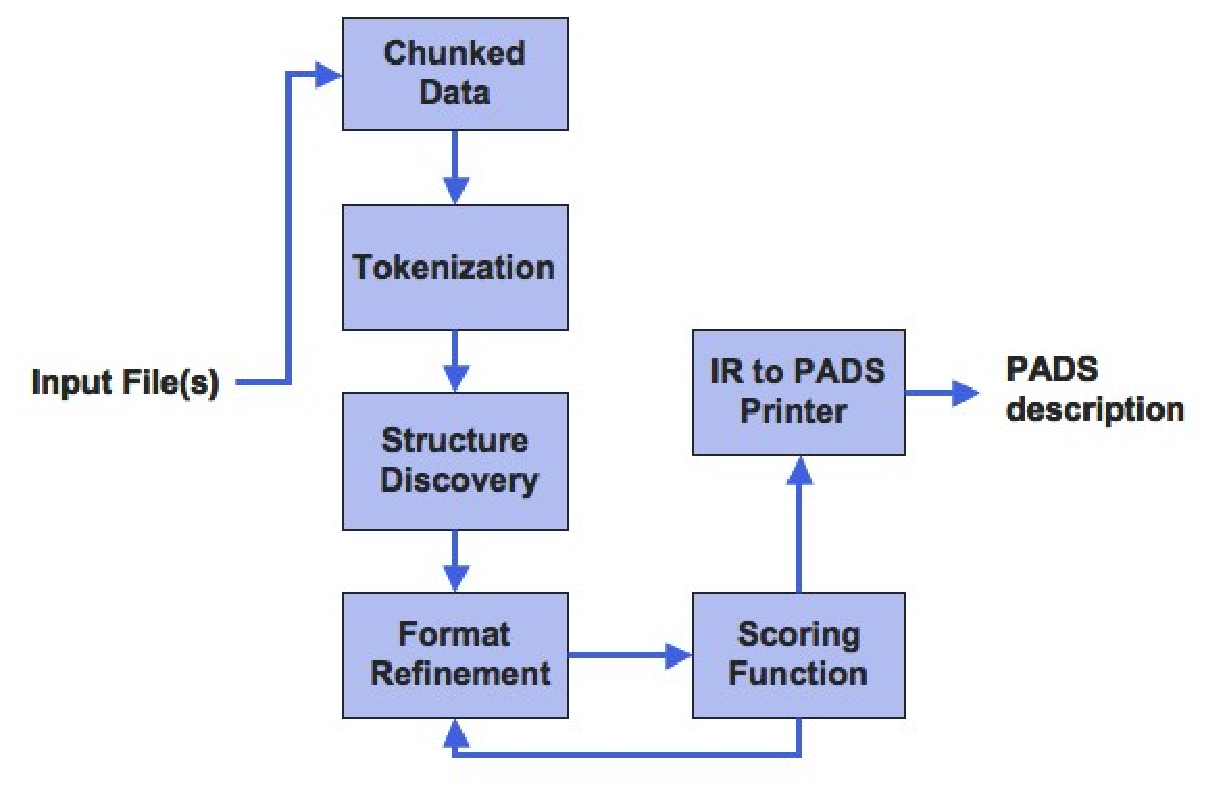
\epsfig{file=archi.eps, width=\columnwidth}
\caption{Architecture of the automatic tool generation engine} \shrink
\label{fig-archi}
\end{center}
\end{figure}

Figure \ref{fig-archi} gives an overview of our automatic
tool generation architecture. The process 
%of generating a suite of data processing tools 
begins with raw data, shown in blue at the top left, which we pipe
into the format inference engine
(circumscribed by dotted lines in the picture).  
This engine produces a syntactically correct \pads{}
description for the data
through a series of phases:
chunking and tokenization, structure discovery, information-theoretic
scoring, and structure refinement.
The system then feeds the generated \pads{} description into the
\pads{} compiler.  The compiler generates libraries, which the system
then links to generic programs for various tasks including a data
analysis tool ({\em a.k.a.,} the {\em accumulator}) and an
ad-hoc-to-\xml{} translator.  At this point, users can apply these
generated tools to their original raw data or to other data with the
same format.
The following subsections describe the main components of the
inference algorithm in more detail.  We 
illustrate the effect of each phase on our running examples and
present the output of some of the generated tools.

\subsection{Chunking and Tokenization}
The learning system first divides the input data, which we refer
to as the {\em training set}, into {\em chunks} as specified by the
user. Intuitively, a chunk is a unit of repetition in the data source.
It is primarily by analyzing sequences of such chunks for commonalities
that we are able to infer data descriptions.  Our tool currently supports
chunking on a line-by-line basis as well as on a file-by-file basis.  

We use a lexer to break each chunk into a series of {\em simple
tokens}, which are intuitively atomic pieces of data such as
numbers, dates, times, alpha-strings, or punctuation symbols.
Every simple token has a corresponding
base type in the \ir{}, though the converse is not true -- there are 
base types that are not used as tokens.  Nevertheless, since
simple tokens have a very close correspondence with base types,
we often use the word {\em token} interchangeably with {\em base type}.
  
Parenthetical syntax, including quotation marks, curly braces, square brackets,
parentheses and \xml{} tags,
often provides very important hints about the structure
of an ad hoc data file.  Therefore, whenever the lexer encounters 
such parentheses, it creates a {\em meta-token}, which is a compound
token that 
represents the pair of parentheses and all the tokens 
within.\footnote{If parenthetical elements
are not well-nested, the meta-tokens are discarded and replaced with
ordinary sequences of simple tokens.}  For example, in Crashreporter.log,
the syntax \cd{[2164]} will yield the meta-token \cd{[*]} instead of
the sequence of three simple tokens \cd{[}, \cd{Pint}, and \cd{]}.  
The structure discovery algorithm eliminates all meta-tokens during
its analysis; whenever it encounters a context consisting of
matching meta-tokens, it cracks open the meta-tokens so it can analyze
the underlying structure.

Our learning system has a default tokenization scheme skewed toward systems
data, but users may specify a different scheme for their own domain
through a configuration file.  For example, computational biologists
may want to add DNA strings {\tt CATTGTT...} to the default tokenization 
scheme.  The configuration file is essentially
a list of name, regular expressions pairs.  The system uses the configuration
file to generate part of the system's lexer, a
collection of new \ir{} base types, and a series of type 
definitions that are incorporated into the final \pads{} specification.  

%% After tokenization, the algorithm enters the {\em structure discovery} 
%% phase.  This phase uses a top-down, divide-and-conquer
%% scheme to guess an approximate, initial format for the data.
%% To assess the quality of this initial approximation, the
%% algorithm computes an information-theoretic {\em score} for the
%% structure.  This score is used in the next phase to guide
%% {\em rewriting rules} that iteratively refine the format.  

%% Once the format has been refined to the extent possible, the resulting
%% \ir{} is printed in \pads{} syntax.  Template programs that use the
%% new description, including the \xml{}-converter, a simple
%% statistics tool we call the {\em accumulator}, a database tool
%% based on Oetiker's RRDTool~\cite{rrdtool}, and the \padx{}
%% query engine, are also all generated at this point.  Hence, starting
%% with data alone, our end-to-end algorithm quickly generates an entire suite
%% of fully functional data processing tools, ready to use at the command line.



% \begin{figure}
% \begin{verbatim}
% def triplet [0-9]{1,3}
% def doublet [0-9]{1,2}
% def hexdoub [0-9a-fA-F]{2}
% ...
% exp Pemail {str1}@{hostname}
% exp Pmac   ({hexdoub}(: | \-)){5}{hexdoub}
% exp PbXML  \<([a-zA-Z])+\>
% exp PeXML  \<\/[^>]+\>
% \end{verbatim}
% \caption{Tiny fragment of the default configuration file. 
% The configuration command {\tt exp} specifies the definition on that
% line should be  ``exported'' to
% the learning tool whereas command {\tt def} implies the definition
% is local and used only in other {\tt exp} or {\tt def} in the
% configuration file.}
% \label {fig:configfile}
% \end{figure}

%% 




%% \begin{figure}
%% \begin{center}
%% \begin{tabular}{|l|l|}
%% \hline
%% Name   &  Description               \\ \hline\hline
%% Pint  &   Integer \\ 
%% Palpha & Alpha-numeric string including '$\_$' and '$-$' \\
%% Pip & IP address \\
%% Pemail & Email address \\
%% Pmac & Mac address \\
%% Pdate & Simple date format \\
%% Ptime & Simple time format \\
%% Ppath & File system path \\
%% Phostname & Hostname \\
%% Purl  & URL \\
%% PbXML & Beginning XML tag \\
%% PeXML & Ending XML tag \\
%% Pother & Punctuation character \\\hline
%% \end{tabular}

%% \caption{Basic token types in default configuration.}
%% \label{figure:base-types}
%% \end{center}
%% \end{figure}
 



%%     *  mention system parameterization for multiple tokenizations for different domains
%%     * mention current skew towards systems data
%%     * ignore problems in this section -- save that for discussion/future work section
%%     * mention stream of tokens generated for running example 

\subsection {Structure Discovery}

Given a collection of tokenized chunks, the goal of the structure
discovery phase is to quickly find a candidate description ``close'' to
a good final solution.  The rewriting phase then analyzes, refines and
tranforms this candidate to produce the final description.
The high-level form of our structure discovery algorithm was
inspired by the work of Arasu and 
Garcia-Molina on information extraction from web pages~\cite{arasu+:sigmod03};
however, the context, goals and algorithmic details of our
work are entirely different.

%However, the details are
%entirely different as Arasu's algorithm operates over well-formed
%\html{} trees whereas our work focuses on the mucky world of ad hoc
%data.

\paragraph*{Structure Discovery Basics.}
Our algorithm operates by analyzing the collection of tokenized chunks
and guessing what the top-level type constructor should be.  Based on
this guess, it partitions the chunks and recursively analyze each partition
to determine the best description for that partition.
Figure~\ref{fig:structure-discovery} outlines the
overall procedure in Pseudo-ML.  The \cd{oracle} function,
whose implementation we hide for now, does most of the hard work by
conjuring one of four different sorts of prophecies.  

The \cd{BaseProphecy} simply reports that the top-level type
constructor is a particular base type.

The \cd{StructProphecy} specifies that the top-level description is a
struct with $k$ fields.  It also
specifies a list, call it \cd{css}, with $k$ elements.  The
$i^{\mathrm{th}}$ element in \cd{css} is the list of chunks
corresponding to the $i^{\mathrm{th}}$ field of the struct.  The
oracle derives these chunk lists from its original input. More
specifically, if the oracle guesses there will be $k$ fields, then
each original chunk is partitioned into $k$ pieces. The
$i^{\mathrm{th}}$ piece of each original chunk is used to recursively
infer the type of the $i^{\mathrm{th}}$ field of the struct.

The \cd{ArrayProphecy} specifies that the top-level structure involves
an array.  However, predicting exactly where an array begins and ends
is difficult, even for the magical oracle.  Consequently, the
algorithm actually generates a three-field struct, where the first
field allows for slop prior to the array, the middle field is the
array itself, and the last field allows for slop after the array.  If
the slop turns out to be unnecessary, the rewriting rules will clean
up the mess in the next phase.

Finally, the \cd{UnionProphecy} specifies that the top-level structure
is a union type with $k$ branches.  Like a \cd{StructProphecy}, the
\cd{UnionProphecy} carries a chunks list, with one element for each
branch of the union.  The algorithm uses each element to recursively
infer a description for the corresponding branch of the union. 
Intuitively, the oracle produces the union chunks list by ``horizontally''
partitioning the input chunks, whereas it partitions struct chunks
``vertically'' along field boundaries. 

As an example, recall the Crashreporter.log data from
Figure~\ref{fig:example}.  Assuming a chunk is a line of data, the two
chunks in the example consist of the token sequences
(recall \cd{[*]} and \cd{(*)} are meta-tokens):

{\small
\begin{verbatim}
Pdate ' ' Ptime ' ' Pint ' ' Palpha [*] ':' ...
'-' ' ' Palpha [*] ':' ' ' Palpha (*) ' ' ...
\end{verbatim}
}%
\noindent
Given these token sequences, 
the oracle will predict that the top-level type constructor is a struct 
with three fields: one for the tokens before the token \cd{[*]}, one
for the \cd{[*]} tokens themslves, and one for the tokens after the token
\cd{[*]}. Based on this determination, the oracle will divide the
original chunks into three sets as follows.

{\small
\begin{verbatim}
Pdate ' ' Ptime ' ' Pint ' ' Palpha        (set 1)       
'-' ' ' Palpha 

[*]                                        (set 2)       
[*]

':' ...                                    (set 3)       
':' ' ' Palpha (*) ' ' ...
\end{verbatim}
}%

\noindent
On recursive analysis of set 1, the oracle again suggests a struct is the top-level type,
generating two more sets of chunks: 

{\small
\begin{verbatim}
Pdate ' ' Ptime ' ' Pint ' '               (set 4)       
'-' ' '

Palpha                                     (set 5)       
Palpha 
\end{verbatim}
}%

\noindent
Now, since every chunk in set 5 contains exactly one base type
token, the recursion bottoms out with the oracle claiming it has
found the base type \cd{Palpha}.  When analyzing set 4, 
the oracle detects insufficient commonality between chunks and decides
the top-most type constructor is a union. It partitions set 4 into
two more sets, with each group containing only 1 chunk (either
\{\cd{Pdate ' ' ...}\} or \{\cd{'-' ' '}\}).  The algorithm analyzes
the first set to determine the type of the first branch of the union
and the second set to determine the second branch of the union.
With no variation in either branch, the algorithm quickly discovers an
accurate type for each. 

Having completely discovered the type of the data in set 1, we turn
our attention to set 2. 
To analyze this set, the algorithm cracks open the \cd{[*]} meta-tokens
to recursively analyze the underlying data, a process which yields 
\cd{struct \{'['; Pint; ']';\}}. Analysis of Set 3 proceeds in a similar 
fashion.

%% The types $T_0$, $T_1$, $T_2$ and $T_3$ are not yet known -- they will
%% be constructed recursively.  $T_0$ is constructed by recursively applying
%% the discovery procedure to the data in the chunks that precedes
%% the first occurrence of \cd{Pdate}.  In this case, there is no such
%% data, so the inference procedure returns the trivial type \cd{Pempty} for
%% $T_0$.  $T_1$ is constructed by applying discovery to the data between
%% \cd{Pdate} and \cd{Ptime}.  Each chunk contains one token in this case,
%% the space token.  Hence the discovery procedure easily decides
%% $T_1$ is \cd{' '}. $T_2$ is discovered by recursively analyzing the following
%% two chunks.
%% {\small
%% \begin{verbatim}
%%    ' ' Pint ' ' Palpha '[' Pint ']' 
%%    ' ' Pint ' ' Palpha '[' Pint ']'
%% \end{verbatim}
%% }
%% \noindent
%% Finally, the structure of $T_3$ is discovered by recursively analyzing 
%% all data following the ':' token.

As a second example, consider the Sirius data from Figure~\ref{fig:example}.
Here the chunks have the following structure:

{\small
\begin{verbatim}
   Pint '|' Pint '|' ... '|' Pint '|' Pint
   Pint '|' Pint '|' ... '|' Palpha Pint '|' Pint
\end{verbatim}
}%

\noindent
In this case, the oracle prophecies that the top-level structure involves
an array and partitions the data into sets of chunks for the
array preamble, the array itself, and the array postamble.  The
preamble chunks all have the form \{\cd{Pint '|'}\} while the
postamble chunks all have the form \{\cd{Pint}\}, so the algorithm
easily determines the corresponding types. The algorithm discovers the
type of the array elements by analyzing the residual list of chunks

{\small
\begin{verbatim}
Pint '|' 
... 
Pint '|' 
Pint '|'
...
Palpha Pint '|'
\end{verbatim}
}%

\noindent
The oracle constructs this chunk list by removing the preamble and
postamble tokens from all input chunks, concatenating the
remaining tokens, and then splitting the resulting list into one chunk
per array element. It does this splitting by assuming that the chunk
for each array element ends with a \cd{'|'} token.  

So far so good, but how does the guessing work?  Why does the
algorithm decide the Sirius data is basically an array but 
Crashreporter.log is a struct? After all, the Sirius chunks all have
a \cd{Pint}, just as all the Crashreporter.log chunks have a bracket
meta-token \cd{[*]}. Likewise, Crashreporter.log contains many occurrences of
the \cd{' '} token, which might serve as
an array separator as the \cd{'|'} token does in the Sirius data.

\begin{figure}
{\small
\begin{verbatim}
type description (* an IR description *)
type chunk       (* a tokenized chunk *)
type chunks = chunk list

(* A top-level description guess *)
datatype prophecy =
   BaseProphecy   of description
 | StructProphecy of chunks list 
 | ArrayProphecy  of chunks * chunks * chunks
 | UnionProphecy  of chunks list

(* Guesses the best top-level description *)
fun oracle : chunks -> prophecy

(* Implements a generic inference algorithm *)
fun discover (cs:chunks) : description =
 case (oracle cs) of
   BaseProphecy b => b

 | StructProphecy css => 
     let Ts = map discover css in
     struct { Ts }

 | ArrayProphecy (csfirst,csbody,cslast) => 
     let Tfirst = discover csfirst in
     let Tbody  = discover csbody  in
     let Tlast  = discover cslast  in
     struct { Tfirst; array { Tbody }; Tlast; }

 | UnionProphecy css => 
     let Ts = map discover css in
     union { Ts }
\end{verbatim}
}
\caption{A generic structure-discovery algorithm in Pseudo-ML.} \shrink
\label{fig:structure-discovery}
\end{figure}


\paragraph*{The Magic.}
To generate the required prophecy for a given list of chunks, the
oracle computes a histogram of the frequencies of all tokens appearing
the input.  
More specifically, the histogram for token $t$
plots the number of chunks (on the $y$-axis)
having a certain number of occurrences of the token (on the $x$-axis). 
Figure~\ref{fig:histograms} presents a number of histograms computed
during analysis of the Crashreporter.log and Sirius chunk lists.

Intuitively, tokens associated 
with histograms with high {\em coverage}, meaning the token appears
in almost every chunk, and {\em narrow} distribution, meaning the variation in
the number of times a token appears in different chunks is low, are
good candidates for defining structs.  Similarly, histograms with
high coverage and {\em wide} distribution are good candidates for defining
arrays.  Finally, histograms with low coverge or intermediate width
represent tokens that form part of a union.  


\begin {figure*}
\begin{center}
\begin{minipage}[t]{0.59\columnwidth}
\epsfig{file=histogram1.eps, width=\columnwidth}
\end{minipage}
\hfill
\begin{minipage}[t]{0.53\columnwidth}
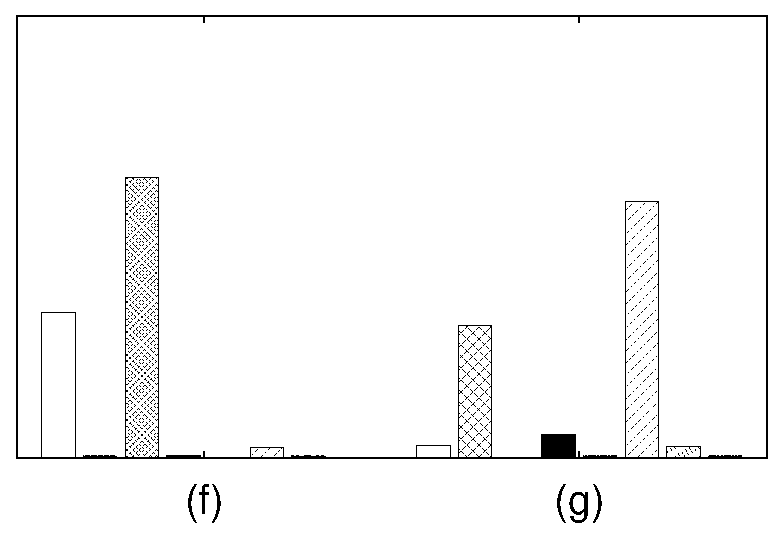
\epsfig{file=histogram2.eps, width=\columnwidth}
\end{minipage}
\hfill
\begin{minipage}[t]{0.295\columnwidth}
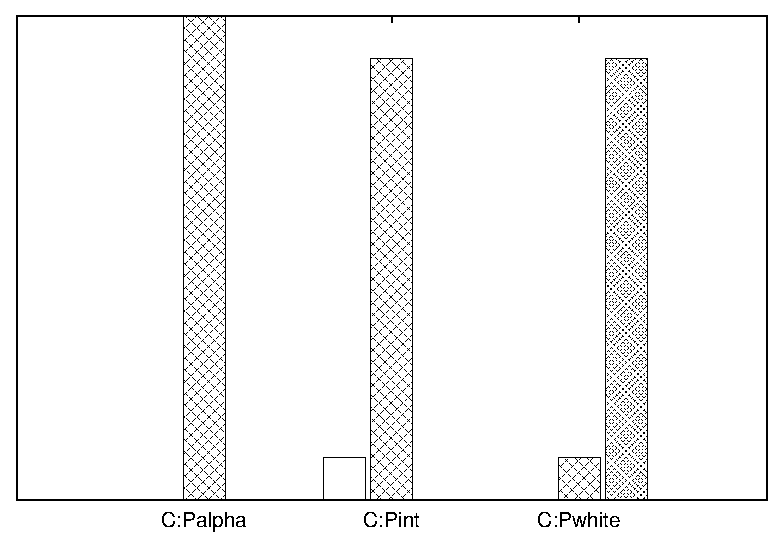
\epsfig{file=histogram3.eps, width=\columnwidth}
\end{minipage}
\hfill
\begin{minipage}[t]{0.59\columnwidth}
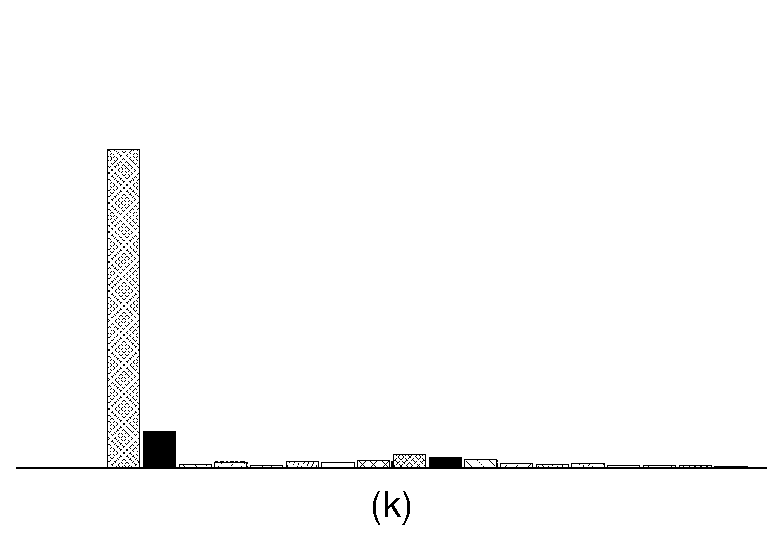
\epsfig{file=histogram4.eps, width=\columnwidth}
\end{minipage}
%
%a) histogram for ' '
%histogram for ':'
%...
%
%Omit telling the reader which histograms are for which tokens in the figure.
%We'll explain in the text...
%
%May 6 of them 3 each from Crashreporter.log and Sirius?
%We'll pick carefully.
\caption{Histograms (a), (b), (c), (d), (e), (f) and
(g) are generated from top-level analysis of Crashreporter.log tokens.
The corresponding tokens are (a) {\tt [*]}, 
(b)  {\tt Pint}, (c) {\tt PDate}, (d) {\tt PTime}, (e) {\tt -}, (f) {\tt Palpha} and
(g) {\tt Pwhite}.  Histograms (h) {\tt Palpha}, (i) {\tt Pint}, and 
(j) {\tt Pwhite} are generated from analysis of Crashreporter.log from
set 1 (the second level of recursion).  Histogram (k) is generated from
top-level analysis of the {\tt |} token from the Sirius data.} \shrink
\label{fig:histograms} 
\end{center}
\end{figure*}

Concretely, consider histogram (a)
from Figure~\ref{fig:histograms}.  It is a perfect struct candidate--
it has a single column that covers 100\% of the records.  Indeed,
this histogram corresponds to the \cd{[*]} token in Crashreporter.log.
Whenever the oracle detects such a histogram, it will always prophecy
a struct and partition the input chunks according to the associated
token. All of the other top-level histograms for Crashreporter.log
contain variation and hence are less certain indicators of data source
structure. 

As a second example, consider the top-level histograms (f), (b) and
(g) for tokens \cd{Palpha}, \cd{Pint} and \cd{Pwhite}, respectively, 
and compare them with the corresponding histograms (h),
(i) and (j) computed for the same tokens from chunk set 1, defined in the
previous subsection.  The histograms for chunk set 1 have far less variation
than the corresponding top-level histograms.  In particular, notice
that histogram (h) for token \cd{Palpha} is a perfect struct histogram
whereas histogram (f) for token \cd{Palpha}
contains a great deal of variation.  This example illustrates the
source of the power of our divide-and-conquer algorithm-- if the
oracle can identify {\em even one token} at a given level as
defining a good partition for the data, the histograms for the next
level down become substantially sharper and more amenable to analysis.

As a third example, consider histogram (k).  This histogram illustrates
the classic pattern for tokens involved in arrays-- it has a very long
tail.  And indeed, the \cd{|} token in the Sirius data does act like a
separator for fields of an array. 

To make the intuitions discussed above precise, we must define a number of
properties of histograms.  First, a histogram $h$ for a token $t$ is a list of pairs
of natural numbers $(x,y)$ where $x$ denotes the token frequency and
$y$ denotes the number of chunks with that frequency.  
All first elements of pairs in the list must be unique.  
The {\em width} of a
histogram ({\em width}($h$)) is the number of elements in the list
excluding the zero-column (\ie{} excluding element $(0,y)$).  
A histogram
$\normal{h}$ is in normal form when the first element of the list is
the zero column and all subsequent elements are sorted in descending
order by the $y$ component.  For example, if $h_1$ is the histogram
$[(0,5), (1,10), (2,25), (3,15)]$ then {\em width}($h_1$) is 3 and its
normal form $\normal{h_1}$ is $[(0,5), (2, 25), (3,15), (1,10)]$.

We often refer to $y$ as the {\em mass} of the element $(x,y)$,
and given a histogram $h$, we refer to the mass of the $i^{\mathrm th}$
element of the list 
using the notation $h[i]$.  For instance, $h_1[3] = 15$ and 
$\normal{h_1}[3] = 10$.  The {\em residual mass} ({\em rm}) of a column $i$ in 
a normalized histogram $h$ is the mass of all the columns to the right of 
$i$ plus the mass of the zero-column.  Mathematically, 
{\em rm}$(\normal{h},i) = \normal{h}[0] + \sum_{j=i+1}^{\mathit{width}(\normal{h})} \normal{h}[j]$.
For example, {\em rm}$(\normal{h_1},1) = 5 + 15 + 10 = 30$.
The residual mass characterizes the ``narrowness''
of a histogram.  Those histograms with low residual mass of the first
column ({\em i.e.,} {\em rm}$(\normal{h_1},1)$ is small) 
are good candidates for structs.

To distinguishing between structs, arrays and unions,
we also need to define the {\em coverage} of a histogram, which
intuitively is the number of chunks containing the corresponding token.
Mathematically, it is simply the sum of the non-zero histogram elements:
{\em coverage}$(\normal{h}) = 
                  \sum_{j=1}^{\mathit{width}(\normal{h})} \normal{h}[j]$.

Finally, our algorithm works better when the oracle considers groups
of tokens with similar distributions together because with very high
probability such tokens form part of the same type constructor. 
To determine when two histograms are {\em similar}, we use
a symmetric form of {\em relative entropy} \cite{Lin91:divergence}.
%\footnote{Suggested by Rob Schapire, personal communication, May 2007.}  
The (plain) relative entropy
of two normalized histograms $\normal{h_1}$ and $\normal{h_2}$, 
written \relativee{\normal{h_1}}{\normal{h_2}}, is
defined as follows.
\[
 \relativee{\normal{h_1}}{\normal{h_2}} 
   = \sum_{j=1}^{\mathit{width}(\normal{h_1})} \normal{h_1}[j]*log(\normal{h_1}[j]/\normal{h_2}[j])
\]
To create a symmetric form, we first find the average of the two
histograms in question (written $\addh{h_1}{h_2}$)
by summing corresponding columns and dividing by two.  This technique
prevents the denominator from being zero in the 
final relative entropy computation.  Using this definition, the symmetric
relative entropy is:
\[
 \srelativee{\normal{h_1}}{\normal{h_2}} 
   = \frac{1}{2}  \relativee{\normal{h_1}}{\addh{\normal{h_1}}{\normal{h_2}}}
   +  \frac{1}{2}  \relativee{\normal{h_2}}{\addh{\normal{h_1}}{\normal{h_2}}}
\]

Now that we have defined the relevant properties of histograms,
we can explain how the oracle prophecies given a list of chunks.

\begin {enumerate}
\item Prophecy a base type when each chunk contains the same simple
  token. If each chunk contains the same meta-token, prophecy a struct
  with three fields: one for the left paren, one for the body, and one
  for the right paren.

\item Otherwise, compute normalized histograms for the input and group
  related ones into clusters using agglomerative clustering:  A
  histogram $h_1$ belongs to group $G$ provided there exists another
  histogram $h_2$ in $G$ such  that
  $\srelativee{\normal{h_1}}{\normal{h_2}} <  \mathrm{ClusterTolerance}$.  
  where $\mathrm{ClusterTolerance}$ is a parameter of the algorithm. We do not
  require all histograms in a cluster to 
  have precisely the same histogram to allow for errors in the data.
  A histogram dissimilar to all others will form its own group.
  We have found a $\mathrm{ClusterTolerance}$ of 0.01 is effective.  

\item Determine if a struct exists by first ranking the groups by the
  minimum residual mass of all the histograms in each group. Find the first group in this
  ordering with histograms $h$ satisfying the following criteria:
\begin {itemize}
\item $\mathit{rm}(h) < \mathrm{MaxMass}$
\item $\mathit{coverage}(h) > \mathrm{MinCoverage}$
\end{itemize}
where constants $\mathrm{MaxMass}$ and $\mathrm{MinCoverage}$ are
parameters of the algorithm.  
This process favors groups of histograms with high
coverage and narrow distribution.  
If histograms $h_1$, \ldots, $h_n$ from
group $G$ satisfy the struct criteria, the oracle will prophecy some
form of struct. It uses the histograms $h_1$, \ldots, $h_n$ and the associated
tokens $t_1$, \ldots, $t_n$ to calculate the number of fields and the
corresponding chunk lists.  We call $t_1$, \ldots, $t_n$ the {\em
  identified} tokens for the input.
Intuitively, for each input chunk, the oracle puts
all tokens upto but not including the first token $t$ from the set of
identifed tokens into the chunk list for the first field.  It puts $t$ in
the chunk list for the second field. It puts all tokens upto the next
identified token into the chunk list for the third field and so on. Of
course, the identified tokens need not appear in the same order in all
input chunks, nor in fact must they all appear at all.  To handle
this variation when it occurs, the oracle prophecies a union instead
of a struct, with one branch per token ordering and one branch for all
input chunks that do not have the full set of identified tokens.


\item Identify an array by sorting all groups in descending 
order by coverage of the highest coverage histogram in the group.
Find the first group in this ordering with any histograms that satisfy
the following minimum criteria:
\begin {itemize}
\item $\mathit{width}(h) > 3$
\item $\mathit{coverage}(h) > \mathrm{MinCoverage}$
\end{itemize}
This process favors histograms with wide distribution and high coverage.
If histograms $h_1$, \ldots, $h_n$ with corresponding tokens 
$t_1$, \ldots, $t_n$ satisfy the array critera, the oracle will
prophecy an array.   It will 
partition each input chunk into (1) a preamble subsequence 
that contains the first occurrence of each identified token, 
(2) a set of element subsequences, with each subsequence containing
one occurrence of the identified tokens, and
(3) a postamble subsequence that contains any remaining tokens from
the input chunk.

\item If no other prophecy applies, identify a union. Partition
  the input chunks according to the first token in each chunk. 
\end{enumerate}

%%     *  role = quickly find a description in the "approximate area" of the correct description
%%     * explain structure of a generic "top-down" inference algorithm -- perhaps give pseudocode
%%     * explain our heuristics: generation of histograms, choice of struct, array, union, base type
%%     * grouping construct (introduce additional example as needed)
%%     * show (part of?) description of running example 

\subsection {Information-Theoretic Scoring}
\label{sec:score}

The goal of the scoring function is to assess the quality of any
inferred description.  This quality metric guides decisions concerning
which rewriting rules to use to refine and transform a candidate
description, as explained in the following section.

Intuitively, a good description is one that is both {\em compact} and
yet {\em precise}.  There are trivial descriptions of any data source
that are highly compact ({\em e.g.,} the description that says
the data source is a string terminated by end of file) or
perfectly precise ({\em e.g.,} the data itself abstracts nothing and
therefore serves as its own description).  A good scoring function
carefully balances these two opposing constraints.  As is common
in machine learning, we have defined a scoring function based on the
{\em Minimum Description Length Principle} (MDL), which states that
a good description is one that minimizes the cost (in bits) of transmitting
the data.  This is accomplished by minimizing 
the sum of the cost of transmitting
the syntax of the description ($\costdescription{T}$)
plus the cost of transmitting the data 
relative to the information known given the description
($\costdata{T}{d_1,\ldots,d_k}$).  Mathematically,
if $T$ is a description and $d_1,\ldots,d_k$ are representations of
the $k$ chunks in our training set, parsed according to $T$, then the 
total cost in bits is:
\[
\totalcost{T}{d_1,\ldots,d_k} = \costdescription{T} + \costdata{T}{d_1,\ldots,d_k}
\]

%\paragraph*{The cost of transmitting a type.}
The cost of transmitting a type, measured in bits, is defined in 
Figure~\ref{fig:cost-type}.  In general, the cost of transmitting
a type is the cost of transmitting the sort of type ({\em i.e.,}\cd{struct},
\cd{union}, \cd{enum}, etc.) plus the cost of transmitting all subcomponents
of the type.  For example, the cost of transmitting any base type
$b(p_1,\ldots,p_k)$ is $ \cardt + \sum_{i=1}^{k} \costparam{p_i}$,
where $\cardt$ is the log of the number of different sorts of type 
constructors (24 of them in the \ir{} presented in this paper)
and $\costparam{p}$ is the cost of encoding the parameter $p$.
The cost of encoding variables, constants and parameters is not
shown in the figure, but is perfectly natural.  For instance, the cost of
encoding an ASCII character is 8 bits.  The cost of encoding a string
is the cost of encoding its length (assumed to be a 32-bit quantity)
plus the cost of encoding each character in turn.

The cost of encoding data relative to selected types is presented in 
Figure~\ref{fig:cost-data}.  At the top of the figure,
we present the cost of encoding all data
chunks relative to the type $T$; it is simply the sum of encoding
each individual chunk relative to $T$.  

In the middle of the figure,
we present the cost of encoding a chunk relative to one of the integer base 
types; other base types are handled similarly.  Notice that the cost of 
encoding an integer relative to the constant type \cd{PintConst} is
zero.  The reason is that the type itself contains all information
necessary to reconstruct the integer -- no data at all need be encoded.
The cost of encoding data relative to \cd{Pint32} or \cd{Pint64} types 
is simply 32 or 64 bits.  Finally, we artificially set the cost of
ranged types \cd{PintRanged}$(p_{min},p_{max})$ to be infinity.
Our experiments reveal that attempting to define integer types with
minimum and maximum values usually leads to overfitting of the data.
We nevertheless retain \cd{PintRanged} types in our \ir{} to encode
the range of values found during the value-space analysis.  During the
rewriting phase, this range information is used to rewrite \cd{PintRanged}
into other integer types.  Since the
cost of encoding \cd{PintRanged} is so high, the appropriate rewriting is 
guaranteed to be applied.  In the future, we may emit this range information
as comments in the generated descriptions.

The last section of Figure~\ref{fig:cost-data} presents the cost of
encoding data relative to selected type constructors.  For example,
the cost of encoding a \cd{struct} is the sum of the costs of encoding
it's component parts.  The cost of encoding a \cd{union} is the cost
of encoding the branch number ($log(k)$ if the union has $k$ branches)
plus the cost of encoding the branch itself.  The cost of encoding
an \cd{enum} is the cost of encoding it's tag only -- given the tag,
the underlying data is determined by the type.  The cost of encoding
a \cd{switch} is the cost of encoding the branch only -- the tag need not
be encoded because it is determined.

\begin{figure}
Miscellaneous definitions:
\[
\begin{array}{@{\,}l@{\,}c@{\,}l}
\cardt &=& \mbox{log of the number of type constructors in the \ir{}}
\end{array}
\]
Cost of transmitting constants and parameters:
\[
\begin {array} {@{}l@{\,}c@{\,}l}
\costchar{a}  &=& \mbox{Cost of transmitting character } a \\
\coststring{s}  &=& \mbox{Cost of transmitting string } s \\
\costint{i}  &=& \mbox{Cost of transmitting integer } i \\
\costconst{c}  &=& \mbox{Cost of transmitting constant } c \\
\costvar{x} &=& \mbox{Cost of transmitting variable } \\
\costparam{p}  &=& \mbox{Cost of transmitting parameter } p \\
\end{array}
\]
Cost of transmitting a type:
\[
\begin{array}{@{}l@{\,}c@{\,}l}
\costdescription{b(p_1,\ldots,p_k)} &=& 
  \cardt + \sum_{i=1}^{k} \costparam{p_i} \\
\costdescription{x{:}b(p_1,\ldots,p_k)} &=& 
  \cardt + \costvar{x} + \sum_{i=1}^{k} \costparam{p_i} \\
\costdescription{\mathtt{struct \{} T_1;\ldots ;T_k; \mathtt{\}}} &=& 
  \cardt + \sum_{i=1}^{k} \costdescription{T_i} \\
\costdescription{\mathtt{union \{} T_1; \ldots ;T_k; \mathtt{\}}} &=& 
  \cardt + \sum_{i=1}^{k} \costdescription{T_i} \\
\costdescription{\mathtt{enum \{} c_1,\ldots,c_k \mathtt{\}}} &=& 
  \cardt + \sum_{i=1}^{k} \costconst{c_i} \\
\end{array}
\]

\caption {Cost of transmitting a type, selected rules}
\label{fig:cost-type}
\end{figure}

\begin{figure}
Cost of encoding all training data relative to a type:
\[
\begin{array}{@{}lcl}
\costdata{T}{d_1,\ldots,d_k} &=& \sum_{i=1}^{k} \adc{T}{d_i} \\
\end{array}
\]
Cost of encoding a single chunk relative to selected base types:
\[
\begin{array}{@{}lcl}
\adc{\mathtt{PintConst}(p)}{i}      &=& 0 \\
\adc{\mathtt{Pint32}}{i}            &=& 32 \\
\adc{\mathtt{Pint64}}{i}            &=& 64 \\
\adc{\mathtt{PintRanged}(p_{min},p_{max})}{i} &=& \infty \\
\end{array}
\]
Cost of encoding a single chunk relative to selected types:

{\em needs more space in between definitions... cannot figure out how
to add it properly without another whole new line
in between definitions...}

\begin{tabbing}
XXXX\=XXXX\=\+\kill
$\adc{\mathtt{struct \{} T_1;\ldots T_k; \mathtt{\}}}{(d_1,\ldots,d_k)}$ \\
  \> $= \sum_{i=1}^{k} \adc{T_i}{d_i}$ \\ 
$\adc{\mathtt{union \{} T_1;\ldots T_k; \mathtt{\}}}{in_i(d)}$ \\            
  \> $= \mathtt{log}(k) + \adc{T_i}{d}$ \\
$\adc{\mathtt{enum \{} c_1;\ldots c_k; \mathtt{\}}}{in_i(c)}$ \\            
  \> $= \mathtt{log}(k)$ \vspace{3pt} \\
$\adc{
\mathtt{switch}\; x \; 
  \mathtt{of \{} 
    c_1 \mathtt{=>} T_1; \ldots  
    c_k \mathtt{=>} T_k; 
  \mathtt{\}}
}{in_i(d)}$ \\ 
  \> $= \adc{T_i}{d}$ \\
\end{tabbing}


\caption {Cost of transmitting data relative to a type, selected rules}
\label{fig:cost-data}
\end{figure}

\subsection {Structure Refinement}

%\documentclass[fleqn]{article}
\usepackage{code}
\newcommand{\struct}[1]{{\tt struct}\{#1\}}
\newcommand{\union}[1]{{\tt union}\{#1\}}
\newcommand{\enum}[1]{{\tt enum}\{#1\}}
\newcommand{\parray}[1]{{\tt array}\{#1\}}
\newcommand{\arrayFW}[2]{{\tt arrayFW}\{#1\}[#2]}
\newcommand{\switch}[2]{{\tt switch}(#1)\{#2\}}
\newcommand{\option}[1]{{\tt option}\{#1\}}
\newcommand{\goto}{\Rightarrow}
\begin{document}
\section{Rewriting Rules}
\subsection*{Data independent rules}
\begin{enumerate}
\item Singleton structs and unions.
\[
\struct{T} \goto T
\]
\[
\struct{} \goto \bot 
\]
\[
\union{T} \goto T
\]
\[
\union{} \goto \bot 
\]

\item Struct and union clean-up
\[
\struct{T_1; \ldots; T_i; \bot; T_j; \ldots; T_n} \goto
\struct{T_1; \ldots; T_i; T_j; \ldots; T_n} 
\] 
\[
\struct{T_1; \ldots; T_i; \emptyset; T_j; \ldots; T_n} \goto
\struct{T_1; \ldots; T_i; T_j; \ldots; T_n} 
\] 

\[
\union{T_1; \ldots; T_i; \bot; T_j; \ldots; T_n} \goto
\union{T_1; \ldots; T_i; T_j; \ldots; T_n} 
\] 
\[
\union{T_1; \ldots; T_i; \emptyset; T_j; \ldots; T_n} \goto
\union{T_1; \ldots; T_i; T_j; \ldots; T_n; \emptyset} 
\]
\noindent where $\emptyset$ means {\tt Pempty}.

\item Union to option
\[
\union{T; \emptyset} \goto \option{T}
\]
\[
\union{\emptyset; T} \goto \option{T}
\]

\item Unnest structs and unions
\begin{eqnarray*}
&& \struct{pretypes; \struct{T_1; \ldots; T_n}; posttypes} \goto \\
&& \struct{pretypes; T_1; \ldots; T_n; posttypes}
\end{eqnarray*}
\begin{eqnarray*}
&&\union{pretypes; \union{T_1; \ldots; T_n}; posttypes} \goto \\
&&\union{pretypes; T_1; \ldots; T_n; posttypes}
\end{eqnarray*}

\item Uniform struct to fixed-length array
\[
\struct{T_1; \ldots; T_n} \goto \arrayFW{T_1}{n}
\]
\noindent if $T_1 = \ldots = T_n$ and $n>=3$.

\item Common prefix or postfix in union branches
\begin{eqnarray*}
&&\union{\struct{T; posttypes_1}; \struct{T, posttypes_2}} \goto \\
&&\struct{T; \union{\struct{posttypes_1}; \struct{posttypes_2}}}
\end{eqnarray*}
\begin{eqnarray*}
&&\union{\struct{T; posttypes}; T} \goto \\
&&\struct{T; \union{\struct{posttypes}; \emptyset}}
\end{eqnarray*}
\begin{eqnarray*}
&&\union{\struct{pretypes_1; T}; \struct{pretypes_2; T}} \goto \\
&&\struct{\union{\struct{pretypes_1}; \struct{pretypes_2}}; T}
\end{eqnarray*}
\begin{eqnarray*}
&&\union{\struct{pretypes; T}; T} \goto \\
&&\struct{\union{\struct{pretypes}; \emptyset}; T}
\end{eqnarray*}

\item {Get floating number number}
\[
\union{{\tt Pint}; {\tt Pfloat}} \goto {\tt Pfloat}
\]

\end{enumerate}

\subsection*{Data dependent rules}
\begin{enumerate}
\item Get floating point number
\begin{eqnarray*}
&& \struct{pretypes; {\tt Pint}(x); {\tt PstringConst ('.')}; {\tt Pint}(y); posttypes} \goto \\
&& \struct{pretypes; {\tt Pfloat}; posttypes}
\end{eqnarray*}
\noindent if $y \ge 0$.
\begin{eqnarray*}
&& \struct{pretypes; {\tt Pint}(x); \option{\struct{{\tt PstringConst ('.')}; {\tt Pint}(y)}}; posttypes} \goto \\
&& \struct{pretypes; {\tt Pfloat}; posttypes}
\end{eqnarray*}
\noindent if $y \ge 0$.

\item Discover negative numbers
\begin{eqnarray*}
&& \struct{pretypes; {\tt Pother}; {\tt PstringConst}('-'); {\tt Pint}(x); posttypes} \goto \\
&& \struct{pretypes; {\tt Pother}; {\tt Pint}; posttypes}
\end{eqnarray*}
\noindent if $x \ge 0$.
\begin{eqnarray*}
&& \struct{pretypes; {\tt Pother}; {\tt PstringConst}('-'); {\tt Pfloat}(x); posttypes} \goto \\
&& \struct{pretypes; {\tt Pother}; {\tt Pfloat}; posttypes}
\end{eqnarray*}
\noindent if $x \ge 0$.
\begin{eqnarray*}
&& \struct{pretypes; {\tt Pother}; \option{{\tt PstringConst}('-')}; {\tt Pint}(x); posttypes} \goto \\
&& \struct{pretypes; {\tt Pother}; {\tt Pint}'; posttypes}
\end{eqnarray*}
\noindent if $x \ge 0$.
\begin{eqnarray*}
&& \struct{pretypes; {\tt Pother}; {\tt \option{PstringConst}('-')}; {\tt Pfloat}(x); posttypes} \goto \\
&& \struct{pretypes; {\tt Pother}; {\tt Pfloat}'; posttypes}
\end{eqnarray*}
\noindent if $x \ge 0$.

\item Unique base types to constant
\[
{\tt Pint}(x) \goto {\tt PintConst(c)}~~ {\rm if}~~ x = c.
\]
\[
{\tt Palpha}(x) \goto {\tt PstringConst(c)}~~ {\rm if}~~ x = c.
\]
\[
{\tt Pstring}(x) \goto {\tt PstringConst(c)}~~ {\rm if}~~ x = c.
\]
\[
{\tt Pother}(x) \goto {\tt PstringConst(c)}~~ {\rm if}~~ x = c.
\]


\item Combine adjacent constant strings
\begin{eqnarray*}
&& \struct{pretypes; {\tt PstringConst (c_1)}; {\tt PstringConst(c_2)}; posttypes} \goto \\
&& \struct{pretypes; {\tt PstringConst (c_1 + c_2)}; posttypes} 
\end{eqnarray*}

\item Refine enums and ranges
\[
{\tt Pstring}(x) \goto \enum{s_1; \ldots; s_k} ~~
{\rm if}~ x~ \in \{s_1, \ldots, s_l\}.
\]
\[
{\tt Pint}(x) \goto {\tt Pint32} ~~
{\rm if}~ 0 \le x~ < 2^{32}.
\]
\[
{\tt Pint}(x) \goto {\tt Pint64} ~~
{\rm if}~ 2^{32} \le x~ < 2^{64}.
\]

\[
{\tt Pint}(x) \goto {\tt PintRanged}(min,~ max) ~~
{\rm if}~ min \le x~ \le max.
\]
\item Union to switch
\begin{eqnarray*}
&&\struct{pretypes; b(x); midtypes; \union{T_1; \ldots; T_n}; posttypes} \goto \\
&&\struct{pretypes, b(x); midtypes; \switch{x}{s_1 \goto T_1; \ldots; s_n \goto T_n}; posttypes}
\end{eqnarray*}
\noindent where $\forall i \in [i,~ n],~ inj_i(\union{T_1; \ldots; T_n}) {\rm implies}~ x = s_i$.

\end{enumerate}

\end{document}


%    *  role = starting with the candidate structure, search for nearby descriptions that optimize an information theoretic scoring function
%    * explain the 3 parts: value independent, value dependent, value independent
%    * give (partial) list of rules used -- we need to work on notation for explaining these rules
%    * illustrate several transformations using the running example
%    * compare example after rewriting to the example from subsection 3.4 above
%    * optional subsubsection: theory suggesting our algorithm is "correct" (we'd need a semantics for our IR then)

The purpose of the structure refinement phase is to improve
the candidate structure produced by the structure discovery phase. We
formulate the structure refinement problem as a generalized search
through description space starting with the candidate produced by
structure discovery. The
objective of the search is to find the description that minimizes
the information-theoretic scoring function.

\paragraph*{Rewriting rules}
In order to move around in description space, we define a number of 
description rewriting rules. The general form of the rule is
\[T \goto T', ~~ {\rm if~ some~ constraint~} p(T)~ {\rm is~ satisfied,}\]
where $T$ is a type, or sub-structure, and $T'$ is the type after the
transition.  Some rules are unconditional and thus free of constraints.
There are two kinds of rewriting rules: (1) data-independent rules which
transform a type based exclusively on the syntax of the description; 
and (2) data-dependent
rules which transform a type based on both the syntax of the description
and on properties of the training data
parsed by this type.  In general, 
the data independent rules aim to rearrange and merge portions
of the structure while the data dependent rules seek to identify 
constant fields and enumerations, and to establish relationships 
between different parts of the structure.

In Figure \ref{fig:rules}, we present a selection of the
data independent and data dependent rules used in the refinement phase.
Many rules have been omitted and some have been simplified for succinctness.
%In these rules,
%let $T_{punc}$ be any type that describes punctuation or white space character%s.
When $T\setof{X}$ appears in a pattern on the left-hand side of a rewriting
rule, $X$ is bound to the set of data representations resulting
from using $T$ to parse the appropriate part of each chunk from the training
set. Furthermore, let $card(X)$ be the cardinality of the set $X$, 
and let $X(i)$ be the data representation resulting
from parsing the $i^{th}$ chunk in the training set. Finally, given a union
value $\mathtt{in}_j(v)$, we define $tag(\mathtt{in}_j(v))$ to be $j$.

\begin{figure*}
\begin{center}
\framebox{
\noindent
\begin{minipage}[t]{\columnwidth}
\paragraph*{Data independent rules}
\begin{enumerate}
\item Singleton structs and unions \\
$
\irstruct{T} \goto T  \qquad\qquad\quad \irunion{T} \goto T
$\\ \\
$
\irstruct{} \goto \Pempty  \qquad\quad\quad \irunion{} \goto \Pvoid 
$
\item Struct and union clean-up\\
$
\irstruct{pre\_types; \Pvoid; post\_types} \goto \Pvoid
$\\ \\ 
$
\irstruct{pre\_types; \Pempty; post\_types} \goto \\
\sskip \irstruct{pre\_types; post\_types}
$\\ \\ 
$
\irunion{pre\_types; \Pvoid; post\_types} \goto \\
\sskip \irunion{pre\_types; post\_types} 
$
%$
%\irunion{pre\_types; \Pempty; post\_types} \goto \\
%\sskip \irunion{pre\_types; post\_types; \Pempty} 
%$
% \item Union to option\\
% $
% \irunion{T; \Pempty} \goto \iroption{T}
% $\\ \\
% $
% \irunion{\Pempty; T} \goto \iroption{T}
% $
% \item Unnest structs and unions\\
% $
% \irstruct{pre\_types; \irstruct{mid\_types}; post\_types} \goto \\
% \sskip \irstruct{pre\_types; mid\_types; post\_types}
% $\\ \\
% $
% \irunion{pre\_types; \irunion{mid\_types}; post\_types} \goto \\
% \sskip \irunion{pre\_types; mid\_types; post\_types}
% $
\item Uniform struct to fixed-length array\\
$
\irstruct{T_1; \ldots; T_n} \goto \irarrayFW{T_1}{n}
$\\ 
\noindent if $n \ge 3$ and $\forall i \in [1,~ n],~ j \in [1,~ n]:~ T_i = T_j$.

\item Common postfix in union branches \\
% $
% \irunion{\irstruct{T; post\_types_1}; \\
% \sskip \irstruct{T, post\_types_2}} \goto \\
% \sskip \irstruct{T; \irunion{\irstruct{post\_types_1}; \\
% \sskip \irstruct{post\_types_2}}}
% $\\ \\
% $
% \irunion{\irstruct{T; post\_types}; T} \goto\\
% \sskip \irstruct{T; \iroption{\irstruct{post\_types}}}
% $\\ \\
$
\irunion{\irstruct{pre\_types_1; T}; \\
\sskip \irstruct{pre\_types_2; T}} \goto \\
\sskip \irstruct{\irunion{\irstruct{pre\_types_1}; \\
\sskip \irstruct{pre\_types_2}}; T}
$\\ \\
$
\irunion{\irstruct{pre\_types; T}; T} \goto \\
\sskip \irstruct{\iroption{\irstruct{pre\_types}}; T}
$

\item Combine adjacent constant strings \\
$
\irstruct{pre\_types; {\tt PstringConst (c_1)}; \\
\sskip {\tt PstringConst(c_2)}; post\_types} \goto \\
\sskip \irstruct{pre\_types; {\tt PstringConst (c_1 {\makeatletter \tt @} c_2)}; post\_types} 
$

% \item {Get floating number number}\\
% $
% \irunion{{\tt Pint}; {\tt Pfloat}} \goto {\tt Pfloat}
% $ 

\end{enumerate}
\end{minipage}
\hfill
\begin{minipage}[t]{\columnwidth}
\paragraph*{Data dependent rules}
\begin{enumerate}
% \item Get floating point number \\
% $
% \irstruct{pre\_types; {\tt Pint}\setof{X}; {\tt PstringConst ('.')};  \\
% \sskip {\tt Pint}\setof{Y}; post\_types} \goto \\
% \sskip \irstruct{pre\_types; {\tt Pfloat}; post\_types}
% $\\ 
% \noindent if $\forall y \in Y:~ y \ge 0$. \\
% \\
% $
% \irstruct{pre\_types; {\tt Pint}\setof{X}; \\
% \sskip \iroption{\irstruct{{\tt PstringConst ('.')};  \\
% \sskip {\tt Pint}\setof{Y}}}; post\_types} \goto \\
% \sskip \irstruct{pre\_types; {\tt Pfloat}; post\_types}
% $ \\
% \noindent if $\forall y \in Y:~ y \ge 0$. 

% \item Discover negative numbers\\
% $
% \irstruct{pre\_types; T_{punc}; {\tt PstringConst}('-');\\
% \sskip {\tt Pint} \setof{X}; post\_types} \goto \\
% \sskip \irstruct{pre\_types; T_{punc}; {\tt Pint}; post\_types}
% $\\ 
% \noindent if $\forall x \in X:~ x \ge 0$. \\
% \\
% $
%  \irstruct{pre\_types; T_{punc}; {\tt PstringConst}('-'); \\
% \sskip {\tt Pfloat}\setof{X}; post\_types} \goto \\
% \sskip \irstruct{pre\_types; T_{punc}; {\tt Pfloat}; post\_types}
% $\\ 
% \noindent if $\forall x \in X:~ x \ge 0$.\\
% \\
% $
%  \irstruct{pre\_types; T_{punc}; \iroption{{\tt PstringConst}('-')}; \\
% \sskip {\tt Pint}(x); post\_types} \goto \\
% \sskip \irstruct{pre\_types; T_{punc}; {\tt Pnat}; post\_types}
% $\\
% \noindent if $\forall x \in X:~ x \ge 0$.\\
% \\
% $
% \irstruct{pre\_types; T_{punc}; {\tt \iroption{PstringConst}('-')}; \\
% \sskip {\tt Pfloat}(x); post\_types} \goto \\
% \sskip  \irstruct{pre\_types; T_{punc}; {\tt Preal}; post\_types}
% $\\
% \noindent if $\forall x \in X:~ x \ge 0$.

\item Base type with unique values to constant \\
$
{\tt Pint}\setof{X} \goto {\tt PintConst(c)} \\
$
{\rm if} $\forall x \in X:~ x = c$. 
\\ \\
$
{\tt Palpha}\setof{X} \goto {\tt PstringConst(c)} \\
$
{\rm if} $\forall x \in X:~ x = c$.
\\ \\
$
{\tt Pstring}\setof{X} \goto {\tt PstringConst(c)} \\
$
{\rm if} $\forall x \in X:~ x = c$.
\\ \\
$
{\tt Pother}\setof{X} \goto {\tt PstringConst(c)} \\ 
$
{\rm if} $\forall x \in X:~ x = c$.

\item Refine enums and ranges \\
$
{\tt Pstring}\setof{X} \goto \irenum{s_1; \ldots; s_k} \\
$
{\rm if}~ $\forall x \in X:~ x~ \in \{s_1, \ldots, s_k\}$.
\\ \\
$
{\tt Pint}\setof{X} \goto {\tt Pint32} \\
$
{\rm if} $\forall x \in X:~ 0 \le x~ < 2^{32}$.
% $
% {\tt Pint}\setof{X} \goto {\tt Pint64} \\
% $
% {\rm if} $\forall x \in X:~ 2^{32} \le x~ < 2^{64}$.
% \\ \\
% $
% {\tt Pint}\setof{X} \goto {\tt PintRanged}(min,~ max) \\
% $
% {\rm if}~ $\forall x \in X:~ min \le x~ \le max$.

\item Union to switch \\
$
\irstruct{pre\_types; \irenum{c_1; \ldots; c_n}\setof{X}; mid\_types; \\
\sskip \irunion{T_1; \ldots; T_n}\setof{Y}; post\_types}\\
\goto \\
\irstruct{pre\_types, z:\irenum{c_1; \ldots; c_n}; mid\_types; \\
\sskip \irswitch{z}{c_1 \goto T_{\Pi(1)}; \ldots; c_n \goto T_{\Pi(n)}}; post\_types}
$\\ 
\noindent where $z$ is a fresh variable, and there exists a permutation $\Pi$, s.t.  $\forall i \in [1,~ card(X)]$, $\Pi(tag(X(i)))=tag(Y(i))$.
\end{enumerate}
\end{minipage}
}
\end{center}
\caption{Selected and simplified rewriting rules} \label{fig:rules}
\end{figure*}

\paragraph*{The Search.}
The core of the rewriting system is 
a recursive, depth-first, greedy search procedure. 
By ``depth-first,'' we mean the algorithm begins by refining the 
children of any structured type before
the structure itself. When refining a type, it selects a rule that 
would {\em minimize} the information-theoretic score of the resulting
structure and applies it to the structure.  It iterates this process until
no further reduction in the score is possible, and at
that time, structure $T$ is said to be {\em stable}.

\begin{figure}
{\small 
\begin{verbatim}
(* a rewriting rule *)
type rule : description -> description  

(* all relevant rules in a list *)
val rules : rule list 

(* measure the score for a type *)
fun score : description -> float

(* find the type with best score from a list *)
fun best: description list -> description

(* improve the given type by one rewriting rule *)
fun oneStep (T:description) : description =
 let all = map (fn rule => rule T) rules in
 let top = best all                      in
 if (score top) < (score T) then
   oneStep top
 else
   T

(* main function to refine an IR description *) 
fun refine (T:description) : description =
  let T' = case T of
      base b => b
    | struct { Ts } => struct { map refine Ts }
    | union { Ts } => union { map refine Ts }
    | switch x of { vTs } => 
       switch x of 
         { map (fn (v, t) => (v, refine t)) vTs }
    | array { T } => 
              array { refine T }
    | option { T } => option { refine T } in
  oneStep T'
\end{verbatim}
}
\caption{Generic local optimization algorithm in Pseudo-ML}
\label{fig:refinement}
\end{figure}

The overall algorithm in Figure \ref{fig:refinement} is applied three
times in succession. 
The first time, the algorithm quickly reduces the initial structure to 
a much simpler, more manageably-sized structure by using
the data-independent rules {\em only}. The second time, data dependent
rules are used refine the base types to constant values and enumerations, etc,
and establish structural dependencies such as switched unions. This phase
requires the value-space analysis described below.
The third time, the set of the data-independent rules
are applied again. The third time is necessary because certain changes
to the base types in phase two, such as the creation of constants, may 
newly enable some of the data-independent rules. 

\paragraph*{Value-space analysis.}
A value-space analysis is performed prior
to applying the data-dependent rules.
This analysis operates by first generating a set of relational tables
from the input data.
Each row of a table corresponds to a chunk and each column of a table
corresponds to either a particular base type from the inferred description,
or to a piece of metadata from the description.  Examples of meta-data
include the tag number from union branches and the length of arrays.
We generate a {\em set} of relational tables as opposed to a single table
as the elements of an array occupy their own separate table (a description 
with no arrays will only have one associated table).
% Here, a number of data dependency tables are generated from the 
% input structure, where each
% column of the tables represent the data values associated with a particular base type 
% in the structure, with some extra columns representing auxilliary information such as
% array sizes and union branching decisions.
 
Every column of every table is analyzed to determine properties,
such as constancy and value range, of the data in that column.
To determine inter-column properties, we have implemented a simplified
variant of the TANE algorithm \cite{TANE-HKPT99},
which identifies functional dependencies between columns in 
relational data.  Because full TANE is too expensive 
(possibly exponential in the number of columns), 
and with insufficient data results in many false positives, 
our simplified algorithm only computes binary dependencies. The 
result of this dependency analysis is used to 
identify switched unions and fixed-size arrays.
%In addition, we also discover all the unary constraints on the base types by
%analysizing every single column in the data tables. We store these unary and
%binary constraint in a constraint map.  A rule can be applied 
%only if the conditions are validated successfully
%against the constraint map. 

\paragraph*{Running example}
To illustrate the refinement process a bit more concretely, let us walk through
a few steps as the system refines the initial structure of the crashreporter.log example.
Let us zoom into the beginning portion of the IR and omit some of the details as follows. 
We annotate each type with two pieces of auxiliary information: id of the node which
can be used as the variable name and the complexity score at this node, 
enclosed in a pair of parenthese. In addition, for Pother base types,
we append the character it binds to in parenthese after the type name.
The intial IR structure of crash reporter looks like this:

{\small
\begin{verbatim}
struct {
  union {
    struct {
      Pdate; Pwhite; Ptime; Pwhite; Pint;  
      Pwhite;          (*)
    };
    struct { 
      "-"; 
      Pwhite;          (*)
    };
  }
  Palpha; "["; Pint; "]";
  union { ... };
};
\end{verbatim}
}


% {\small
% \begin{verbatim}
% struct(BTy_114, 416156.763b) {
%   union(BTy_7, 204984.986b) {
%     struct(BTy_6, 204589.179b) {
%       Pdate (BTy_0, 108004.535b);
%       Pwhite (BTy_1, 809.044b);
%       Ptime (BTy_2, 88802.177b);
%       Pwhite (BTy_3, 809.044b);
%       Pint (BTy_4, 5347.705b);
%       Pwhite (BTy_5, 809.044b);
%     };
%     struct(BTy_10, 388.762b) {
%       Pother (-) (BTy_8, 299.673b);
%       Pwhite (BTy_9, 83.044b);
%     };
%   }
%   Palpha (BTy_11, 23879.044b);
%   Pother ([) (BTy_13, 3336.618b);
%   Pint (BTy_14, 6899.045b);
%   Pother (]) (BTy_15, 3336.618b);
%   union(BTy_63, 173712.822b) {
%     struct(BTy_62, 156487.759b) {
%       ...
%     };
%     struct(BTy_113, 17218.019b) {
%       ...
%     };
%   };
% };
% \end{verbatim}
% }

% {\small
% \begin{verbatim}
% struct(BTy_114, 416156.509b) {
%   struct(BTy_115, 204984.732b) {
%     union(BTy_7, 204091.634b) {
%       struct(BTy_6, 203779.872b) {
%         Pdate (BTy_0, 108004.535b);
%         Pwhite (BTy_1, 809.044b);
%         Ptime (BTy_2, 88802.177b);
%         Pwhite (BTy_3, 809.044b);
%         Pint (BTy_4, 5347.705b);
%       };
%       struct(BTy_10, 304.718b) {
%         Pother (-) (BTy_8, 299.673b);
%       };
%     }
%     Pwhite (BTy_5, 887.044b);
%   }
%   ...
% };
% \end{verbatim}
% }

% Note that we end up with an undesirable situation in BTy\_10 where a struct 
% contains just one element. That will be fixed in Phase three as we shall see.
% Next, the "unnest struct and union" rule kicks in to flatten struct BTy\_114 to
% the following.

In the first, value-independent phase of rewriting, 
the common trailing white space marked {\tt (*) } above is
pulled out of the unions and flattened inside the surrounding
struct using the ``common postfix in union'' rule.  This 
transformation leaves behind the unnecessarily verbose
single-element struct on the line marked {\tt (**)}.  However, this
will be transformed into the more compact constant 
string {\tt "-"} in phase three of rewriting.  This rewriting
phase also pulls colon and whitespace characters out of the 
trailing union (marked {\tt (**)}).

{\small
\begin{verbatim}
struct {
  union {
    struct { Pdate; Pwhite; Ptime; Pwhite; Pint; };
    struct { "-" };                 (**)
  }
  Pwhite;                           (*)
  Palpha; "["; Pint; "]"; ":"; Pwhite; (***)
  union { ... };
};
\end{verbatim}
}

% struct(BTy_114, 416056.899b) {
%     union(BTy_7, 204091.634b) {
%       struct(BTy_6, 203779.872b) {
%         Pdate (BTy_0, 108004.535b);
%         Pwhite (BTy_1, 809.044b);
%         Ptime (BTy_2, 88802.177b);
%         Pwhite (BTy_3, 809.044b);
%         Pint (BTy_4, 5347.705b);
%       };
%       struct(BTy_10, 304.718b) {
%         Pother (-) (BTy_8, 299.673b);
%       };
%     Pwhite (BTy_5, 887.044b);
%     ...
%   }
%   ...
% };

In the second rewriting phase, 
data-dependent rules 3 and 4 are applied to base types to 
create a number of constants and enums.
Moreover, a data dependency is discovered between the
newly introduced enumeration involving {\tt "crashdump"},
{\tt "mach\_msg"}, {\em etc.}, and the structure of the following message.
Hence, a switched union is also introduced.
Notice that the switched union is switching on a different enum 
than the hand-written IR in Figure \ref{fig:crashreporter:ir}, because
the inference algorithm has decided on a different way of partitioning
the chunks. Nonetheless, both of these descriptions are
correct.


{\small
\begin{verbatim}
struct {
  union {
    struct { Pdate; " "; Ptime; " "; 2006; };
    struct { "-" };
  };
  " "; enum {"crashreporterd", "crashdump"};
  "["; PintRanged [120...29874]; "]"; ":"; " ";
  x19:enum {"crashdump", "mach_msg", "Finished", 
            "Started", "Unable", "Failed"};
  switch x19 of { ... };
};
\end{verbatim}
}

% struct(BTy_114, 304553.986b) {
%   union(BTy_7, 196876.315b) {
%     struct(BTy_6, 196853.182b) {
%       Pdate (BTy_0, 108004.535b);
%       " " (BTy_1, 11.044b);
%       Ptime (BTy_2, 88802.177b);
%       " " (BTy_3, 11.044b);
%       2006 (BTy_4, 17.015b);
%     };
%     struct(BTy_10 39, 16.089b) {
%       "-" (BTy_8 39, 11.044b);
%     };
%   };
%   " " (BTy_5, 11.044b);
%   enum {"crashreporterd", "crashdump"}(BTy_11, 156.133b);
%   "[" (BTy_13, 11.044b);
%   Pint [120...29874] (BTy_14, 6580.450b);
%   "]" (BTy_10, 11.044b);
%   ":" (BTy_12, 11.044b);
%   " " (BTy_13, 11.044b);
%   enum {"crashdump", "mach_msg", "Finished", "Started", 
%         "Unable", "Failed"} (BTy_19, 317.405b);
%   union(BTy_63, 100570.505b) {
%     ...
%   };
% };


% Further, data dependency is discovered between type BTy\_19
% and the union BTy\_63, and thus the latter is converted to
% a switched union as follows.

% {\small
% \begin{verbatim}
% struct(BTy_114, 304552.986b) {
%   ...
%   enum {"crashdump", "mach_msg", "Finished", "Started", 
%         "Unable", "Failed"} (BTy_19, 317.405b);
%   switch BTy_14 of (BTy_63, 100569.505b) {
%     enum {"Failed", "Finished", "Started"}   => 
%       struct(BTy_57, 99696.280b) {
%        ...
%       };
%     enum {"Unable", "crashdump", "mach_msg"} =>
%       struct(BTy_108, 867.181b) {
%        ...
%       };
%   };
% };
% \end{verbatim}
% }

In the third and final phase, 
data independent rule 5  is applied to combine many constants 
and rule 1 is used to flatten the singleton struct. The final IR follows.

{\small
\begin{verbatim}
struct {
  union {
    struct { Pdate; " "; Ptime; " "; 2006; };
    "-";
  };
  " "; enum {"crashreporterd", "crashdump"};
  "["; Pint32; "]: ";
  x19:enum {"crashdump", "mach_msg", "Finished", 
        "Started", "Unable", "Failed"};
  switch x19 of { ... };
  };
};
\end{verbatim}
}


% {\small
% \begin{verbatim}
% struct(BTy_114, 304537.855b) {
%   union(BTy_7, 196876.315b) {
%     struct(BTy_6, 196853.182b) {
%       Pdate (BTy_0, 108004.535b);
%       " " (BTy_1, 11.044b);
%       Ptime (BTy_2, 88802.177b);
%       " " (BTy_3, 11.044b);
%       2006 (BTy_4, 17.015b);
%     };
%     "-" (BTy_8 39, 11.044b);
%   };
%   " " (BTy_5, 11.044b);
%   enum {"crashreporterd", "crashdump"}(BTy_11, 156.133b);
%   "[" (BTy_13, 11.044b);
%   Pint [120...29874] (BTy_14, 6580.450b);
%   "]: " (BTy_10, 23.044b);
%   enum {"crashdump", "mach_msg", "Finished", "Started", 
%         "Unable", "Failed"} (BTy_19, 317.405b);
%   switch BTy_14 of (BTy_63, 100569.505b) {
%     enum {"Failed", "Finished", "Started"}   => 
%       struct(BTy_57, 99696.280b) {
%        ...
%       };
%     enum {"Unable", "crashdump", "mach_msg"} =>
%       struct(BTy_108, 867.181b) {
%        ...
%       };
%   };
% };
% \end{verbatim}
% }

Comparing this final result with the initial description, one can see that
the structure refinement significately simplified the IR and improved the
complexity score; and with
the explicit constants and enums, the description is a lot more
informative than before.
 

\subsection {Final Products}

The previous subsections outline the central technical elements of our
algorithms.  The main tasks remaining include converting the internal
representation into a syntactically correct \pads{} description, feeding
the generated description to the \pads{} compiler and producing a 
collection of scripts that conveniently package the freshly-generated 
libraries with the \pads{} run-time system and tools.  At the end of 
this process, users have a number of programming libraries
and many powerful tools at their disposal.
Perhaps the most powerful tools are the \padx{} query 
engine~\cite{fernandez+:padx} and the \xml{} converter, which allow  
users to write arbitrary XQueries over the data source
or to convert the data to \xml{} for use by other software. Other
useful tools include the accumulator tool, mentioned earlier,
converters to translate data into a form suitable for
loading into a relational database or Excel spreadsheet, and
a custom graphing tool that pushes data into \cd{gnuplot} for data
visualization.
\figref{fig:final-products} gives snapshots of the output of a couple
of these tools. 

\begin{figure}
\begin{center}
{\small
\begin{verbatim}
<Struct_114>
  <var_7>
    <var_6>
      <var_0><val>Wed Jun 21</val></var_0>
      <var_2><val>10:24:44</val></var_2>
      <var_4><val>2006</val></var_4>
    </var_6>
  </var_7>
  <var_11><val>crashdump</val></var_11>
  <var_14><val>1524</val></var_14>
  <var_19><val>crashdump</val></var_19>
  <var_63>
    <var_113_crashdump19>
      <var_68>
      </var_68>
      <var_73><val>started</val></var_73>
      <var_75>
      </var_75>
    </var_113_crashdump19>
  </var_63>
</Struct_114>
\end{verbatim}
}

(a)

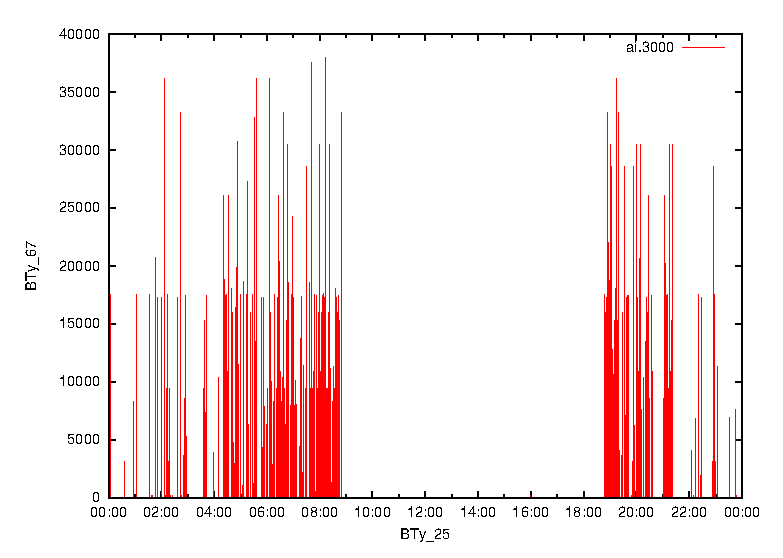
\epsfig{file=ai.3000.eps, width=0.9\columnwidth} 

(b)
\caption{(a) XML output snipet of crashreporter.log  (b) ai.3000 web transaction volumn 
during 19:00 - 08:55(+1 day) visualization} \shrink
\end{center}
\label{fig:final-products}
\end{figure}

%Of course, the end products of the inference algorithm 
%also include the generated description and the
%programming libraries including parser and printer.


\section{Experimental Evaluation}
\label{sec:exp}
\section{Evaluation}
\label{sec:eval}
The following experiments were done on a PowerBook G4 with a 1.67GHz PowerPC
CPU and 2G memory running on Mac OS X 10.4. 
Table \ref{tab:results} compares the performance results between
the original \learnpads{} system and the incremental system. 
The benchmarks used are 12 system logs with various sizes. Column 2
shows the number of lines in each log. The time columns record the total
running time in seconds, and the TC columns record the type complexity
of the final description learned. In general, lower type complexity means
more compact description. For the first 7 benchmarks which are smaller
and simpler, the initial learn size is 100 lines and the 
incremental learn size is 100 lines. For the last 5 benchmarks, 
the initial learn size is 500 lines while the incremental size remains
100 lines. Where it takes more than half an hour for the original \learnpads{}
system to learn a description, a ``-'' is put in those cells to 
indicate there is no result.

\begin{table}[th]
\begin{tabular}{|c|c|c|c|c|c|}\hline
& & \multicolumn{2}{|c|}{original} & \multicolumn{2}{|c|}{incremental} \\ \cline{3-6}
\raisebox{1.5ex}[0pt]{Formats} & \raisebox{1.5ex}[0pt]{Lines} &
	Time & TC & Time & TC \\ \hline \hline
ai.3000	&	3000	& 32	& 412.6	& 2.2	& 571.0	\\ \hline
asl.log  &	1500	& 31.9	& 960.1	& 23.9 	& 1393.3 \\ \hline
apache.txt  &	2087	& 83.9 & 1746.1 & 7.9 	& 2527.6 \\ \hline
access\_log  &	8188 	& 134.5	& 351.2	& 2.9	& 321.2	\\ \hline
error\_log  &	4510	& 101.7	& 101.9	& 0.9	& 107.9 \\ \hline
interface.loop & 1253	& 54.0	& 741.4	& 1.9	& 1053.7 \\ \hline
ai.big	&	57368	& -	& -	& 30	& 533.9 \\ \hline
pws	&	 17365	& -	& - 	& 133  & 5869 \\ \hline
coblitz.access & 9421   & -	& -	& 31.9 & 3005.2 \\ \hline
access.exlog & 260796 	& -	& -	& 610 & 3088.3 \\ \hline
debug\_getbig & 550409   & -	& -	& 668 & 9008.1 \\ \hline
dbg\_req\_redirect & 302554 & -	& -	& 1852 & 17567.7 \\ \hline
\end{tabular}
\caption{Execution times (secs) and type complexity (bits)} 
\label{tab:results}
\end{table}


% - parse metric
% - initial learn size and chunk size - these can affect results
% - update chunk by chunk 
% - optimizations/heuristics
%   due to performance concerns:
%   - memoization
%   - the clean function (to reduce the number of parses)
%   - control of aggregate size
%   - parses cut-off: kill a parse if it has more than n consecutive failures in a struct
%   due to quality of description concerns (and also performance)
%   - deterministic unions
%   - longest match in arrays
%   - merge adjacent const strings (only punctuation and white spaces)
%   - error recovery
%
%- Experiments
%	1) comparison with old LearnPADS on several large datasets (ai.3000, asl.log, apache.txt, access\_log, error\_log, interface.loop)
%	   compare exec time and type complexity. For increment, use
%	   initial learn chunk of 100 and incremental error chunks of 100
%	2) use ai format, do a table with 1000 5000 10000,...,1M miles
%	   using orig learning system and the new system with various optimization turned on and off.
%



\section{Discussion}
\label{sec:discussion}

\paragraph*{Dealing with errors.}  
In 1967, Gold~\cite{gold:inference}
proved that learning a grammar for any remotely
sophisticated class of languages, such as the regular languages, 
is impossible if one is only given positive 
example data.\footnote{A positive example is a data source
known to be in the grammar to be learned.  
A negative example is one known {\em not} to be in the target grammar.
Learning with positive examples and negative examples is possible.
Unfortunately, given that data analysts are unlikely to have access to
ad hoc data that they know {\em does not} 
satisfy the format they are interested in learning,
we are forced to tackle the more difficult problem of learning from 
positive examples only.}
Given this negative theoretical result, and the practical fact
that it is hard to be sure that training data
is sufficiently rich to witness all possible variation in the data,
errors in inference are inevitable.  Fortunately, however, detecting
and recovering from errors in ad hoc data is one of the primary strengths
of the \pads{} system.  

To determine exactly how accurate an
inferred description is on any new data source, a user may run the
accumulator tool.  This tool catalogs exactly how many deviations
from the description there were overall in the data source
as well as the error rate in every individual field.
Hence, using this tool, a programmer can immediately and reliably
determine the effectiveness of inference for their data.
If there is a serious 
problem, the user can easily edit the generated description by hand
-- identification of a problem field, a minor
edit and recompilation of tools might just take 5 minutes.  Hence,
even imperfectly-generated descriptions have great value in terms of
improving programmer productivity.  Moreover, all \pads{}-generated 
parsers and tools
have error detection, representation and recovery techniques.
For instance, when converting data to \xml{}, errors encountered
are represented explicitly in the \xml{} document, allowing users to query
the data for errors if they choose.  Before graphing ad hoc data,
an analyst may use the accumulator tool to check if any errors occur
in the fields to be graphed.  If not, there is no reason to edit
the description at all -- graphing the correct fields may proceed 
immediately.

\paragraph*{Future work.}  
Discovering tokens like ``IP address'' and ``date'' is highly beneficial
as such tokens act as compact, highly 
descriptive, human-readable abstractions. 
Unfortunately, these tokens are also often 
mutually ambiguous.  For instance, an IP address, a 
floating point number 
and a phone number can all be represented as some number of digits 
separated by periods.  At the moment, we disambiguate between them 
in the same way that lex does, by taking the first, longest match. 
In select cases, when we cannot disambiguate in the tokenization phase, we
try to correct problems using domain-specific rewriting rules in the 
structure refinement phase.    
To improve tokenization in the future, we plan to look at learning
probabilistic models of a broad range of token types.  
We also
intend to explore finding new tokens from the data itself,
possibly by identifying abrupt changes in entropy~\cite{hutchens98finding}.

%From an experimental perspective,

% Hence, while our system allows users to
% customize the tokenization scheme through a configuration file,
% this customization requires work, and 
% for the computational biologist not accustomed to writing or 
% reading regular expressions, it creates a barrier to usage.  
% Moreover,
% since tokenization ambiguities are often unavoidable, even after tweaking
% tokenization configurations, system results
% are dependent upon our simplistic disambiguation 
% scheme.\footnote{We disambiguate
% like lex does, taking the first, longest match in the token list.}  
% Indeed, to avoid ambiguities that arise from having
% floating-point numbers be tokens, we do not identify floats during
% the tokenization face, but instead introduce floats through a number of 
% custom
% rewriting rules in the rewriting phase.  

% At the moment, we see two possible solutions to this problem.  The
% first solution is to attempt to identify new tokens from the data 
% source being learned, perhaps by identifying significant changes in entropy
% as suggested by.  This 

% thoughts on problems with tokenization; information theory; partial
% descriptions; user interface; recursion; more experimentation with a
% broader range of formats


\section{Related Work}
\label{sec:related}
\section{Related Work}\label{sec:related}




\section{Conclusions}
\label{sec:conclusion}
The explosive growth of the internet has made monitoring and managing
data systems distributed across wide-area networks increasingly
important.  The possibility of partial failure and the need to
synchronize makes such code tedious and difficult to write correctly,
particularly for data experts whose skills are in domains other than
networking. In this paper, we describe the \padsd{} system, which
allows users to declaratively specify their data systems and then
generate a wide-variety of tools for manipulating the data: from
stand-alone tools, to simple libraries for writing their own analyses,
to generic libraries for building new generic tools.  We precisely
specify the meaning of our language via a sound denotational
semantics and show via experimentation that the system has
acceptable performance overheads.


\section*{Acknowledgments}

Our work benefited greatly from thoughts and comments by
Alex Aiken, David Blei, David Burke, John Launchbury, Chris Ramming, 
Rob Schapire
and the organizers and attendees of the CAGI 2007 workshop on Grammar
induction.

This material is based upon work 
supported by DARPA under grant FA8750-07-C-0014
and the NSF
   under grants 0612147 and 0615062.
Any opinions, findings, and conclusions or recommendations
   expressed in this material are those of the authors and do not
   necessarily reflect the views of DARPA or the NSF.

\bibliographystyle{abbrv}
\bibliography{pads}

%%\newpage
\appendix

\section{Example Data and Descriptions}
\label{app:examples}


%%% Local Variables: 
%%% mode: latex
%%% TeX-master: "semantics"
%%% End: 


\end{document}

%%% Local Variables:
%%% mode: outline-minor
%%% End:

